\documentclass{book}
\usepackage[a4paper,top=2.5cm,bottom=2.5cm,left=2.5cm,right=2.5cm]{geometry}
\usepackage{makeidx}
\usepackage{natbib}
\usepackage{graphicx}
\usepackage{multicol}
\usepackage{float}
\usepackage{listings}
\usepackage{color}
\usepackage{ifthen}
\usepackage[table]{xcolor}
\usepackage{textcomp}
\usepackage{alltt}
\usepackage{ifpdf}
\ifpdf
\usepackage[pdftex,
            pagebackref=true,
            colorlinks=true,
            linkcolor=blue,
            unicode
           ]{hyperref}
\else
\usepackage[ps2pdf,
            pagebackref=true,
            colorlinks=true,
            linkcolor=blue,
            unicode
           ]{hyperref}
\usepackage{pspicture}
\fi
\usepackage[utf8]{inputenc}
\usepackage{mathptmx}
\usepackage[scaled=.90]{helvet}
\usepackage{courier}
\usepackage{sectsty}
\usepackage[titles]{tocloft}
\usepackage{doxygen}
\lstset{language=C++,inputencoding=utf8,basicstyle=\footnotesize,breaklines=true,breakatwhitespace=true,tabsize=8,numbers=left }
\makeindex
\setcounter{tocdepth}{3}
\renewcommand{\footrulewidth}{0.4pt}
\renewcommand{\familydefault}{\sfdefault}
\hfuzz=15pt
\setlength{\emergencystretch}{15pt}
\hbadness=750
\tolerance=750
\begin{document}
\hypersetup{pageanchor=false,citecolor=blue}
\begin{titlepage}
\vspace*{7cm}
\begin{center}
{\Large Cyto\-Sim \\[1ex]\large 0.\-5 }\\
\vspace*{1cm}
{\large Generated by Doxygen 1.8.0}\\
\vspace*{0.5cm}
{\small Mon Apr 9 2012 15:08:58}\\
\end{center}
\end{titlepage}
\clearemptydoublepage
\pagenumbering{roman}
\tableofcontents
\clearemptydoublepage
\pagenumbering{arabic}
\hypersetup{pageanchor=true,citecolor=blue}
\chapter{The Main Page for the Cyto\-Sim software package}
\label{index}\hypertarget{index}{}\hypertarget{index_intro_sec}{}\section{Introduction}\label{index_intro_sec}
Cell motility plays a key role in human biology and disease, contributing ubiquitously to such important processes as embryonic development, wound repair and cancer metastasis. Papoian laboratory is interested in gaining deeper understanding of the physical chemistry behind these complex, far-\/from-\/equilibrium mechano-\/chemical processes. His approach and model, named Mechano-\/chemical Dynamics of Active Networks, 3rd Generation (M\+E\+D\+Y\+A\+N3), is based on combining stochastic reaction-\/diffusion treatment of cellular biochemical processes with polymer physics of cytoskeletal filament network growth, while explicitly coupling chemistry and mechanics.

Papoian laboratory has developed {\bfseries M3\+S\+Y\+M}, a software package based on the M\+E\+D\+Y\+A\+N3 model, to simulate growth dynamics of actin based filamentous networks {\itshape in vitro} and {\itshape in vivo}. Recent papers where {\bfseries M3\+S\+Y\+M} or its predecessor, {\bfseries Stoch\+Tools}, were used can be found on the publication section of \href{http://papoian.chem.umd.edu/}{\tt the Papoian group's main web page\+:}. The {\bfseries M3\+S\+Y\+M} package can also be extended to simulate the dynamics of any active matter network.\hypertarget{index_install_sec}{}\section{Installation}\label{index_install_sec}
\hypertarget{index_step1}{}\subsection{Step 1\+: Prerequisites}\label{index_step1}
The following software packages need to be installed first\+:


\begin{DoxyItemize}
\item Boost 1.\+49
\item G\+S\+L ...
\end{DoxyItemize}\hypertarget{index_step2}{}\subsection{Step 2\+: Installation of M3\+S\+Y\+M itself}\label{index_step2}
Untar the {\bfseries M3\+S\+Y\+M} source code into some directory, enter into the \char`\"{}\+M3\+S\+Y\+M\char`\"{} and execute \char`\"{}make\char`\"{} from the command line. 
\chapter{Class Index}
\section{Class Hierarchy}
This inheritance list is sorted roughly, but not completely, alphabetically\-:\begin{DoxyCompactList}
\item \contentsline{section}{Object}{\pageref{classObject}}{}
\begin{DoxyCompactList}
\item \contentsline{section}{Species}{\pageref{classSpecies}}{}
\begin{DoxyCompactList}
\item \contentsline{section}{S\-Bulk}{\pageref{classSBulk}}{}
\end{DoxyCompactList}
\end{DoxyCompactList}
\item \contentsline{section}{species\-\_\-type\-\_\-tag}{\pageref{structspecies__type__tag}}{}
\item \contentsline{section}{Species\-D\-B}{\pageref{classSpeciesDB}}{}
\item \contentsline{section}{Species\-Factory}{\pageref{classSpeciesFactory}}{}
\end{DoxyCompactList}

\chapter{Class Index}
\section{Class List}
Here are the classes, structs, unions and interfaces with brief descriptions\-:\begin{DoxyCompactList}
\item\contentsline{section}{\hyperlink{classObject}{Object} }{\pageref{classObject}}{}
\item\contentsline{section}{\hyperlink{classSBulk}{S\-Bulk} \\*This class represent Bulk species that have no spatial component, i.\-e. are not connected to any Compartmens }{\pageref{classSBulk}}{}
\item\contentsline{section}{\hyperlink{classSpecies}{Species} }{\pageref{classSpecies}}{}
\item\contentsline{section}{\hyperlink{structspecies__type__tag}{species\-\_\-type\-\_\-tag} \\*Create a tag for the corresponding Species\-Type flywheights }{\pageref{structspecies__type__tag}}{}
\item\contentsline{section}{\hyperlink{classSpeciesDB}{Species\-D\-B} \\*\hyperlink{classSpeciesDB}{Species\-D\-B} should be used for obtaining new objects of the \hyperlink{classSpecies}{Species} hieararchy }{\pageref{classSpeciesDB}}{}
\item\contentsline{section}{\hyperlink{classSpeciesFactory}{Species\-Factory} \\*This is the standard implentation of the \hyperlink{classSpecies}{Species} Factory Method, which can be further subclassed to either specialize or introduce other construction behaviors }{\pageref{classSpeciesFactory}}{}
\end{DoxyCompactList}

\chapter{File Index}
\section{File List}
Here is a list of all files with brief descriptions\-:\begin{DoxyCompactList}
\item\contentsline{section}{Cyto\-Sim/\hyperlink{ChemNRMImpl_8cpp}{Chem\-N\-R\-M\-Impl.\-cpp} }{\pageref{ChemNRMImpl_8cpp}}{}
\item\contentsline{section}{Cyto\-Sim/\hyperlink{ChemNRMImpl_8h}{Chem\-N\-R\-M\-Impl.\-h} }{\pageref{ChemNRMImpl_8h}}{}
\item\contentsline{section}{Cyto\-Sim/\hyperlink{ChemRNode_8h}{Chem\-R\-Node.\-h} }{\pageref{ChemRNode_8h}}{}
\item\contentsline{section}{Cyto\-Sim/\hyperlink{ChemSim_8cpp}{Chem\-Sim.\-cpp} }{\pageref{ChemSim_8cpp}}{}
\item\contentsline{section}{Cyto\-Sim/\hyperlink{ChemSim_8h}{Chem\-Sim.\-h} }{\pageref{ChemSim_8h}}{}
\item\contentsline{section}{Cyto\-Sim/\hyperlink{ChemSimImpl_8h}{Chem\-Sim\-Impl.\-h} }{\pageref{ChemSimImpl_8h}}{}
\item\contentsline{section}{Cyto\-Sim/\hyperlink{common_8cpp}{common.\-cpp} }{\pageref{common_8cpp}}{}
\item\contentsline{section}{Cyto\-Sim/\hyperlink{common_8h}{common.\-h} }{\pageref{common_8h}}{}
\item\contentsline{section}{Cyto\-Sim/\hyperlink{Compartment_8cpp}{Compartment.\-cpp} }{\pageref{Compartment_8cpp}}{}
\item\contentsline{section}{Cyto\-Sim/\hyperlink{Compartment_8h}{Compartment.\-h} }{\pageref{Compartment_8h}}{}
\item\contentsline{section}{Cyto\-Sim/\hyperlink{Component_8cpp}{Component.\-cpp} }{\pageref{Component_8cpp}}{}
\item\contentsline{section}{Cyto\-Sim/\hyperlink{Component_8h}{Component.\-h} }{\pageref{Component_8h}}{}
\item\contentsline{section}{Cyto\-Sim/\hyperlink{Composite_8cpp}{Composite.\-cpp} }{\pageref{Composite_8cpp}}{}
\item\contentsline{section}{Cyto\-Sim/\hyperlink{Composite_8h}{Composite.\-h} }{\pageref{Composite_8h}}{}
\item\contentsline{section}{Cyto\-Sim/\hyperlink{main_8cpp}{main.\-cpp} }{\pageref{main_8cpp}}{}
\item\contentsline{section}{Cyto\-Sim/\hyperlink{Reaction_8cpp}{Reaction.\-cpp} }{\pageref{Reaction_8cpp}}{}
\item\contentsline{section}{Cyto\-Sim/\hyperlink{Reaction_8h}{Reaction.\-h} }{\pageref{Reaction_8h}}{}
\item\contentsline{section}{Cyto\-Sim/\hyperlink{RSpecies_8cpp}{R\-Species.\-cpp} }{\pageref{RSpecies_8cpp}}{}
\item\contentsline{section}{Cyto\-Sim/\hyperlink{RSpecies_8h}{R\-Species.\-h} }{\pageref{RSpecies_8h}}{}
\item\contentsline{section}{Cyto\-Sim/\hyperlink{Species_8cpp}{Species.\-cpp} }{\pageref{Species_8cpp}}{}
\item\contentsline{section}{Cyto\-Sim/\hyperlink{Species_8h}{Species.\-h} \\*This header file will contain defininition of the Species hieararchy and associated D\-B and helper classes }{\pageref{Species_8h}}{}
\item\contentsline{section}{Cyto\-Sim/\hyperlink{System_8cpp}{System.\-cpp} }{\pageref{System_8cpp}}{}
\item\contentsline{section}{Cyto\-Sim/\hyperlink{System_8h}{System.\-h} }{\pageref{System_8h}}{}
\item\contentsline{section}{Cyto\-Sim/\hyperlink{utility_8h}{utility.\-h} }{\pageref{utility_8h}}{}
\item\contentsline{section}{Cyto\-Sim/\hyperlink{Visitor_8h}{Visitor.\-h} }{\pageref{Visitor_8h}}{}
\item\contentsline{section}{Cyto\-Sim/\hyperlink{VisitorConcrete_8h}{Visitor\-Concrete.\-h} }{\pageref{VisitorConcrete_8h}}{}
\end{DoxyCompactList}

\chapter{Class Documentation}
\hypertarget{classObject}{\section{Object Class Reference}
\label{classObject}\index{Object@{Object}}
}


{\ttfamily \#include $<$Object.\-h$>$}



Inheritance diagram for Object\-:\nopagebreak
\begin{figure}[H]
\begin{center}
\leavevmode
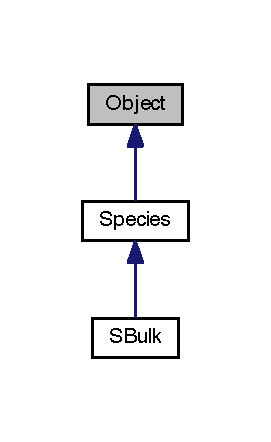
\includegraphics[width=130pt]{classObject__inherit__graph}
\end{center}
\end{figure}
\subsection*{Public Member Functions}
\begin{DoxyCompactItemize}
\item 
\hyperlink{Object_8h_a0b56ddf6ace42572542aae1f2c364e05}{object\-\_\-id} \hyperlink{classObject_a4dd34b912b01d62f8e5aa9bcb4e82e81}{get\-I\-D} ()
\begin{DoxyCompactList}\small\item\em return the object\-\_\-id associated with this object \end{DoxyCompactList}\item 
virtual void \hyperlink{classObject_a3f41123d1b33b22e5eb71fd2794577d9}{write\-Self} (std\-::ofstream \&fout)
\begin{DoxyCompactList}\small\item\em Write the \hyperlink{classObject}{Object} into the provided output filestream, fout. \end{DoxyCompactList}\item 
virtual void \hyperlink{classObject_a7695d57d88356ed2649255a48e4ffdbe}{initialize\-From\-Stream} (std\-::ifstream \&fin)
\begin{DoxyCompactList}\small\item\em initialize the \hyperlink{classObject}{Object} based on the data from the inpute filestream \end{DoxyCompactList}\end{DoxyCompactItemize}
\subsection*{Static Public Member Functions}
\begin{DoxyCompactItemize}
\item 
static \hyperlink{classObject}{Object} $\ast$ \hyperlink{classObject_a0fcfbdfa4439b322c375a5f99c3dfabd}{get\-Objectby\-I\-D} (\hyperlink{Object_8h_a0b56ddf6ace42572542aae1f2c364e05}{object\-\_\-id} id)
\begin{DoxyCompactList}\small\item\em A static method, which should be invoked as,. \end{DoxyCompactList}\end{DoxyCompactItemize}
\subsection*{Protected Member Functions}
\begin{DoxyCompactItemize}
\item 
\hyperlink{classObject_a40860402e64d8008fb42329df7097cdb}{Object} ()
\begin{DoxyCompactList}\small\item\em Default constructor without arguments is the usual way to initialize \hyperlink{classObject}{Object}. \end{DoxyCompactList}\item 
\hyperlink{classObject_a7c0918b6f13db00e14c729dc954d320c}{Object} (\hyperlink{Object_8h_a0b56ddf6ace42572542aae1f2c364e05}{object\-\_\-id} I\-D)
\begin{DoxyCompactList}\small\item\em The main reason for using this constructor is reconstruction of Objects when read from a file (i.\-e. \end{DoxyCompactList}\item 
\hyperlink{classObject}{Object} $\ast$ \hyperlink{classObject_a11a1dd53ef68fc4a1ad8c6175132c8d5}{clone\-Object} ()
\begin{DoxyCompactList}\small\item\em Duplicate the \hyperlink{classObject}{Object} instance. \end{DoxyCompactList}\end{DoxyCompactItemize}


\subsection{Detailed Description}
This is the base class of \hyperlink{classSpecies}{Species}, Reactions, Compartments, Filaments, etc. \begin{DoxyNote}{Note}
A class derived from \hyperlink{classObject}{Object} cannot be copied, but instead should be duplicated in a special way. Classes inherited from \hyperlink{classObject}{Object} need to implement the {\bfseries Persistence interface}, so to be able to write themselves into an output filestream and read themselves from an input filestream 
\end{DoxyNote}


Definition at line 36 of file Object.\-h.



\subsection{Constructor \& Destructor Documentation}
\hypertarget{classObject_a40860402e64d8008fb42329df7097cdb}{\index{Object@{Object}!Object@{Object}}
\index{Object@{Object}!Object@{Object}}
\subsubsection[{Object}]{\setlength{\rightskip}{0pt plus 5cm}{\bf Object\-::\-Object} (
\begin{DoxyParamCaption}
{}
\end{DoxyParamCaption}
)\hspace{0.3cm}{\ttfamily  \mbox{[}inline, protected\mbox{]}}}}\label{classObject_a40860402e64d8008fb42329df7097cdb}


Default constructor without arguments is the usual way to initialize \hyperlink{classObject}{Object}. 



Definition at line 68 of file Object.\-h.



Referenced by clone\-Object().

\hypertarget{classObject_a7c0918b6f13db00e14c729dc954d320c}{\index{Object@{Object}!Object@{Object}}
\index{Object@{Object}!Object@{Object}}
\subsubsection[{Object}]{\setlength{\rightskip}{0pt plus 5cm}{\bf Object\-::\-Object} (
\begin{DoxyParamCaption}
\item[{{\bf object\-\_\-id}}]{I\-D}
\end{DoxyParamCaption}
)\hspace{0.3cm}{\ttfamily  \mbox{[}inline, protected\mbox{]}}}}\label{classObject_a7c0918b6f13db00e14c729dc954d320c}


The main reason for using this constructor is reconstruction of Objects when read from a file (i.\-e. 

to implement persistence). It should not be necessary otherwise. 

Definition at line 77 of file Object.\-h.



\subsection{Member Function Documentation}
\hypertarget{classObject_a11a1dd53ef68fc4a1ad8c6175132c8d5}{\index{Object@{Object}!clone\-Object@{clone\-Object}}
\index{clone\-Object@{clone\-Object}!Object@{Object}}
\subsubsection[{clone\-Object}]{\setlength{\rightskip}{0pt plus 5cm}{\bf Object}$\ast$ {\bf Object\-::clone\-Object} (
\begin{DoxyParamCaption}
{}
\end{DoxyParamCaption}
)\hspace{0.3cm}{\ttfamily  \mbox{[}inline, protected\mbox{]}}}}\label{classObject_a11a1dd53ef68fc4a1ad8c6175132c8d5}


Duplicate the \hyperlink{classObject}{Object} instance. 

Despite its name, the \-\_\-id variable is not duplicated, because all \hyperlink{classObject}{Object} I\-Ds are required to be unique during any time of the program run. 

Definition at line 86 of file Object.\-h.



References Object().

\hypertarget{classObject_a4dd34b912b01d62f8e5aa9bcb4e82e81}{\index{Object@{Object}!get\-I\-D@{get\-I\-D}}
\index{get\-I\-D@{get\-I\-D}!Object@{Object}}
\subsubsection[{get\-I\-D}]{\setlength{\rightskip}{0pt plus 5cm}{\bf object\-\_\-id} {\bf Object\-::get\-I\-D} (
\begin{DoxyParamCaption}
{}
\end{DoxyParamCaption}
)\hspace{0.3cm}{\ttfamily  \mbox{[}inline\mbox{]}}}}\label{classObject_a4dd34b912b01d62f8e5aa9bcb4e82e81}


return the object\-\_\-id associated with this object 



Definition at line 39 of file Object.\-h.

\hypertarget{classObject_a0fcfbdfa4439b322c375a5f99c3dfabd}{\index{Object@{Object}!get\-Objectby\-I\-D@{get\-Objectby\-I\-D}}
\index{get\-Objectby\-I\-D@{get\-Objectby\-I\-D}!Object@{Object}}
\subsubsection[{get\-Objectby\-I\-D}]{\setlength{\rightskip}{0pt plus 5cm}static {\bf Object}$\ast$ {\bf Object\-::get\-Objectby\-I\-D} (
\begin{DoxyParamCaption}
\item[{{\bf object\-\_\-id}}]{id}
\end{DoxyParamCaption}
)\hspace{0.3cm}{\ttfamily  \mbox{[}inline, static\mbox{]}}}}\label{classObject_a0fcfbdfa4439b322c375a5f99c3dfabd}


A static method, which should be invoked as,. 


\begin{DoxyCode}
 object_id ID = 35;
 Object* o = Object::getObjectbyID(ID);
 ...
\end{DoxyCode}
 

Definition at line 47 of file Object.\-h.

\hypertarget{classObject_a7695d57d88356ed2649255a48e4ffdbe}{\index{Object@{Object}!initialize\-From\-Stream@{initialize\-From\-Stream}}
\index{initialize\-From\-Stream@{initialize\-From\-Stream}!Object@{Object}}
\subsubsection[{initialize\-From\-Stream}]{\setlength{\rightskip}{0pt plus 5cm}virtual void {\bf Object\-::initialize\-From\-Stream} (
\begin{DoxyParamCaption}
\item[{std\-::ifstream \&}]{fin}
\end{DoxyParamCaption}
)\hspace{0.3cm}{\ttfamily  \mbox{[}inline, virtual\mbox{]}}}}\label{classObject_a7695d57d88356ed2649255a48e4ffdbe}


initialize the \hyperlink{classObject}{Object} based on the data from the inpute filestream 



Reimplemented in \hyperlink{classSBulk_aade6080b259012cbf1a5a84d64352358}{S\-Bulk}, and \hyperlink{classSpecies_a73ca4b8decc02298a91aff1912f57df4}{Species}.



Definition at line 53 of file Object.\-h.



Referenced by Species\-::initialize\-From\-Stream().

\hypertarget{classObject_a3f41123d1b33b22e5eb71fd2794577d9}{\index{Object@{Object}!write\-Self@{write\-Self}}
\index{write\-Self@{write\-Self}!Object@{Object}}
\subsubsection[{write\-Self}]{\setlength{\rightskip}{0pt plus 5cm}virtual void {\bf Object\-::write\-Self} (
\begin{DoxyParamCaption}
\item[{std\-::ofstream \&}]{fout}
\end{DoxyParamCaption}
)\hspace{0.3cm}{\ttfamily  \mbox{[}inline, virtual\mbox{]}}}}\label{classObject_a3f41123d1b33b22e5eb71fd2794577d9}


Write the \hyperlink{classObject}{Object} into the provided output filestream, fout. 



Reimplemented in \hyperlink{classSBulk_af96d228dfe5348a5a7944b69c3ddf8fa}{S\-Bulk}, and \hyperlink{classSpecies_a8a2ec8930dd89c427245f0013aea9c69}{Species}.



Definition at line 50 of file Object.\-h.



Referenced by Species\-::write\-Self().



The documentation for this class was generated from the following files\-:\begin{DoxyCompactItemize}
\item 
/\-Users/papoian/\-Dropbox/\-Codes/\-Cyto\-Sim/\-Cyto\-Sim/\hyperlink{Object_8h}{Object.\-h}\item 
/\-Users/papoian/\-Dropbox/\-Codes/\-Cyto\-Sim/\-Cyto\-Sim/\hyperlink{Object_8cpp}{Object.\-cpp}\end{DoxyCompactItemize}

\hypertarget{classSBulk}{\section{S\-Bulk Class Reference}
\label{classSBulk}\index{S\-Bulk@{S\-Bulk}}
}


This class represent Bulk species that have no spatial component, i.\-e. are not connected to any Compartmens.  




{\ttfamily \#include $<$Species.\-h$>$}



Inheritance diagram for S\-Bulk\-:
\nopagebreak
\begin{figure}[H]
\begin{center}
\leavevmode
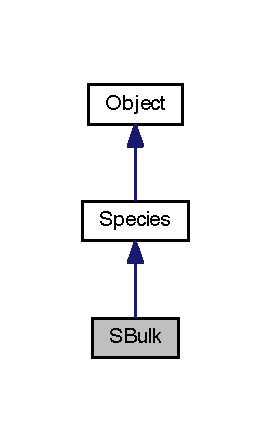
\includegraphics[width=130pt]{classSBulk__inherit__graph}
\end{center}
\end{figure}


Collaboration diagram for S\-Bulk\-:
\nopagebreak
\begin{figure}[H]
\begin{center}
\leavevmode
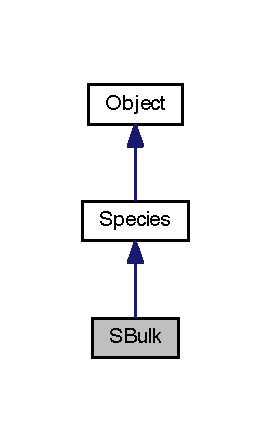
\includegraphics[width=130pt]{classSBulk__coll__graph}
\end{center}
\end{figure}
\subsection*{Public Member Functions}
\begin{DoxyCompactItemize}
\item 
\hyperlink{classSBulk_ad4c6f917b6456d8b6e38ee776419c6c6}{S\-Bulk} (const \hyperlink{Species_8h_af8f3afcc030f67a124aa4a6b5badf495}{Species\-Type} \&name, int N)
\item 
virtual void \hyperlink{classSBulk_af96d228dfe5348a5a7944b69c3ddf8fa}{write\-Self} (std\-::ofstream \&fout)
\begin{DoxyCompactList}\small\item\em Write th class \hyperlink{classSBulk}{S\-Bulk} into the provided output filestream, fout. \end{DoxyCompactList}\item 
virtual void \hyperlink{classSBulk_aade6080b259012cbf1a5a84d64352358}{initialize\-From\-Stream} (std\-::ifstream \&fin)
\begin{DoxyCompactList}\small\item\em initialize the Sbulk based on the data from the inpute filestream \end{DoxyCompactList}\item 
int \hyperlink{classSpecies_a166f138f95713c4fd02dfb47a81b515b}{get\-N} ()
\begin{DoxyCompactList}\small\item\em return the current copy number of this particule \hyperlink{classSpecies}{Species} object \end{DoxyCompactList}\item 
void \hyperlink{classSpecies_af40a72d3e3f8d3cc7bf1dfe209bed39b}{set\-N} (int N)
\begin{DoxyCompactList}\small\item\em param N -\/ an integer argument to set the current copy number of this particule \hyperlink{classSpecies}{Species} object \end{DoxyCompactList}\item 
const \hyperlink{Species_8h_af8f3afcc030f67a124aa4a6b5badf495}{Species\-Type} \& \hyperlink{classSpecies_a7b99d16574deaba7a1f4b60d93f33304}{get\-Type} ()
\begin{DoxyCompactList}\small\item\em return reference to Species\-Type, which should behave as a std\-::string (i.\-e. \char`\"{}\-Arp2/3\char`\"{}) \end{DoxyCompactList}\item 
\hyperlink{Object_8h_a0b56ddf6ace42572542aae1f2c364e05}{object\-\_\-id} \hyperlink{classObject_a4dd34b912b01d62f8e5aa9bcb4e82e81}{get\-I\-D} ()
\begin{DoxyCompactList}\small\item\em return the object\-\_\-id associated with this object \end{DoxyCompactList}\end{DoxyCompactItemize}
\subsection*{Static Public Member Functions}
\begin{DoxyCompactItemize}
\item 
static \hyperlink{classObject}{Object} $\ast$ \hyperlink{classObject_a0fcfbdfa4439b322c375a5f99c3dfabd}{get\-Objectby\-I\-D} (\hyperlink{Object_8h_a0b56ddf6ace42572542aae1f2c364e05}{object\-\_\-id} id)
\begin{DoxyCompactList}\small\item\em A static method, which should be invoked as,. \end{DoxyCompactList}\end{DoxyCompactItemize}
\subsection*{Protected Member Functions}
\begin{DoxyCompactItemize}
\item 
\hyperlink{classObject}{Object} $\ast$ \hyperlink{classObject_a11a1dd53ef68fc4a1ad8c6175132c8d5}{clone\-Object} ()
\begin{DoxyCompactList}\small\item\em Duplicate the \hyperlink{classObject}{Object} instance. \end{DoxyCompactList}\end{DoxyCompactItemize}
\subsection*{Protected Attributes}
\begin{DoxyCompactItemize}
\item 
int \hyperlink{classSpecies_aaf64f0a20dc213a6f03c69e7c3caa43a}{\-\_\-\-N}
\item 
\hyperlink{Species_8h_af8f3afcc030f67a124aa4a6b5badf495}{Species\-Type} \hyperlink{classSpecies_ae80ccbaa2b115cea250b7f87ce517105}{\-\_\-\-Type}
\end{DoxyCompactItemize}


\subsection{Detailed Description}
This class represent Bulk species that have no spatial component, i.\-e. are not connected to any Compartmens. 

Definition at line 81 of file Species.\-h.



\subsection{Constructor \& Destructor Documentation}
\hypertarget{classSBulk_ad4c6f917b6456d8b6e38ee776419c6c6}{\index{S\-Bulk@{S\-Bulk}!S\-Bulk@{S\-Bulk}}
\index{S\-Bulk@{S\-Bulk}!SBulk@{S\-Bulk}}
\subsubsection[{S\-Bulk}]{\setlength{\rightskip}{0pt plus 5cm}{\bf S\-Bulk\-::\-S\-Bulk} (
\begin{DoxyParamCaption}
\item[{const {\bf Species\-Type} \&}]{name, }
\item[{int}]{N}
\end{DoxyParamCaption}
)\hspace{0.3cm}{\ttfamily  \mbox{[}inline\mbox{]}}}}\label{classSBulk_ad4c6f917b6456d8b6e38ee776419c6c6}


Definition at line 83 of file Species.\-h.



\subsection{Member Function Documentation}
\hypertarget{classObject_a11a1dd53ef68fc4a1ad8c6175132c8d5}{\index{S\-Bulk@{S\-Bulk}!clone\-Object@{clone\-Object}}
\index{clone\-Object@{clone\-Object}!SBulk@{S\-Bulk}}
\subsubsection[{clone\-Object}]{\setlength{\rightskip}{0pt plus 5cm}{\bf Object}$\ast$ {\bf Object\-::clone\-Object} (
\begin{DoxyParamCaption}
{}
\end{DoxyParamCaption}
)\hspace{0.3cm}{\ttfamily  \mbox{[}inline, protected, inherited\mbox{]}}}}\label{classObject_a11a1dd53ef68fc4a1ad8c6175132c8d5}


Duplicate the \hyperlink{classObject}{Object} instance. 

Despite its name, the \-\_\-id variable is not duplicated, because all \hyperlink{classObject}{Object} I\-Ds are required to be unique during any time of the program run. 

Definition at line 86 of file Object.\-h.



References Object\-::\-Object().

\hypertarget{classObject_a4dd34b912b01d62f8e5aa9bcb4e82e81}{\index{S\-Bulk@{S\-Bulk}!get\-I\-D@{get\-I\-D}}
\index{get\-I\-D@{get\-I\-D}!SBulk@{S\-Bulk}}
\subsubsection[{get\-I\-D}]{\setlength{\rightskip}{0pt plus 5cm}{\bf object\-\_\-id} {\bf Object\-::get\-I\-D} (
\begin{DoxyParamCaption}
{}
\end{DoxyParamCaption}
)\hspace{0.3cm}{\ttfamily  \mbox{[}inline, inherited\mbox{]}}}}\label{classObject_a4dd34b912b01d62f8e5aa9bcb4e82e81}


return the object\-\_\-id associated with this object 



Definition at line 39 of file Object.\-h.

\hypertarget{classSpecies_a166f138f95713c4fd02dfb47a81b515b}{\index{S\-Bulk@{S\-Bulk}!get\-N@{get\-N}}
\index{get\-N@{get\-N}!SBulk@{S\-Bulk}}
\subsubsection[{get\-N}]{\setlength{\rightskip}{0pt plus 5cm}int {\bf Species\-::get\-N} (
\begin{DoxyParamCaption}
{}
\end{DoxyParamCaption}
)\hspace{0.3cm}{\ttfamily  \mbox{[}inline, inherited\mbox{]}}}}\label{classSpecies_a166f138f95713c4fd02dfb47a81b515b}


return the current copy number of this particule \hyperlink{classSpecies}{Species} object 



Definition at line 48 of file Species.\-h.

\hypertarget{classObject_a0fcfbdfa4439b322c375a5f99c3dfabd}{\index{S\-Bulk@{S\-Bulk}!get\-Objectby\-I\-D@{get\-Objectby\-I\-D}}
\index{get\-Objectby\-I\-D@{get\-Objectby\-I\-D}!SBulk@{S\-Bulk}}
\subsubsection[{get\-Objectby\-I\-D}]{\setlength{\rightskip}{0pt plus 5cm}static {\bf Object}$\ast$ {\bf Object\-::get\-Objectby\-I\-D} (
\begin{DoxyParamCaption}
\item[{{\bf object\-\_\-id}}]{id}
\end{DoxyParamCaption}
)\hspace{0.3cm}{\ttfamily  \mbox{[}inline, static, inherited\mbox{]}}}}\label{classObject_a0fcfbdfa4439b322c375a5f99c3dfabd}


A static method, which should be invoked as,. 


\begin{DoxyCode}
 object_id ID = 35;
 Object* o = Object::getObjectbyID(ID);
 ...
\end{DoxyCode}
 

Definition at line 47 of file Object.\-h.

\hypertarget{classSpecies_a7b99d16574deaba7a1f4b60d93f33304}{\index{S\-Bulk@{S\-Bulk}!get\-Type@{get\-Type}}
\index{get\-Type@{get\-Type}!SBulk@{S\-Bulk}}
\subsubsection[{get\-Type}]{\setlength{\rightskip}{0pt plus 5cm}const {\bf Species\-Type}\& {\bf Species\-::get\-Type} (
\begin{DoxyParamCaption}
{}
\end{DoxyParamCaption}
)\hspace{0.3cm}{\ttfamily  \mbox{[}inline, inherited\mbox{]}}}}\label{classSpecies_a7b99d16574deaba7a1f4b60d93f33304}


return reference to Species\-Type, which should behave as a std\-::string (i.\-e. \char`\"{}\-Arp2/3\char`\"{}) 



Definition at line 54 of file Species.\-h.

\hypertarget{classSBulk_aade6080b259012cbf1a5a84d64352358}{\index{S\-Bulk@{S\-Bulk}!initialize\-From\-Stream@{initialize\-From\-Stream}}
\index{initialize\-From\-Stream@{initialize\-From\-Stream}!SBulk@{S\-Bulk}}
\subsubsection[{initialize\-From\-Stream}]{\setlength{\rightskip}{0pt plus 5cm}virtual void {\bf S\-Bulk\-::initialize\-From\-Stream} (
\begin{DoxyParamCaption}
\item[{std\-::ifstream \&}]{fin}
\end{DoxyParamCaption}
)\hspace{0.3cm}{\ttfamily  \mbox{[}inline, virtual\mbox{]}}}}\label{classSBulk_aade6080b259012cbf1a5a84d64352358}


initialize the Sbulk based on the data from the inpute filestream 



Reimplemented from \hyperlink{classSpecies_a73ca4b8decc02298a91aff1912f57df4}{Species}.



Definition at line 91 of file Species.\-h.



References Species\-::initialize\-From\-Stream().

\hypertarget{classSpecies_af40a72d3e3f8d3cc7bf1dfe209bed39b}{\index{S\-Bulk@{S\-Bulk}!set\-N@{set\-N}}
\index{set\-N@{set\-N}!SBulk@{S\-Bulk}}
\subsubsection[{set\-N}]{\setlength{\rightskip}{0pt plus 5cm}void {\bf Species\-::set\-N} (
\begin{DoxyParamCaption}
\item[{int}]{N}
\end{DoxyParamCaption}
)\hspace{0.3cm}{\ttfamily  \mbox{[}inline, inherited\mbox{]}}}}\label{classSpecies_af40a72d3e3f8d3cc7bf1dfe209bed39b}


param N -\/ an integer argument to set the current copy number of this particule \hyperlink{classSpecies}{Species} object 



Definition at line 51 of file Species.\-h.

\hypertarget{classSBulk_af96d228dfe5348a5a7944b69c3ddf8fa}{\index{S\-Bulk@{S\-Bulk}!write\-Self@{write\-Self}}
\index{write\-Self@{write\-Self}!SBulk@{S\-Bulk}}
\subsubsection[{write\-Self}]{\setlength{\rightskip}{0pt plus 5cm}virtual void {\bf S\-Bulk\-::write\-Self} (
\begin{DoxyParamCaption}
\item[{std\-::ofstream \&}]{fout}
\end{DoxyParamCaption}
)\hspace{0.3cm}{\ttfamily  \mbox{[}inline, virtual\mbox{]}}}}\label{classSBulk_af96d228dfe5348a5a7944b69c3ddf8fa}


Write th class \hyperlink{classSBulk}{S\-Bulk} into the provided output filestream, fout. 



Reimplemented from \hyperlink{classSpecies_a8a2ec8930dd89c427245f0013aea9c69}{Species}.



Definition at line 85 of file Species.\-h.



References Species\-::write\-Self().



Referenced by main().



\subsection{Member Data Documentation}
\hypertarget{classSpecies_aaf64f0a20dc213a6f03c69e7c3caa43a}{\index{S\-Bulk@{S\-Bulk}!\-\_\-\-N@{\-\_\-\-N}}
\index{\-\_\-\-N@{\-\_\-\-N}!SBulk@{S\-Bulk}}
\subsubsection[{\-\_\-\-N}]{\setlength{\rightskip}{0pt plus 5cm}int {\bf Species\-::\-\_\-\-N}\hspace{0.3cm}{\ttfamily  \mbox{[}protected, inherited\mbox{]}}}}\label{classSpecies_aaf64f0a20dc213a6f03c69e7c3caa43a}


Definition at line 75 of file Species.\-h.

\hypertarget{classSpecies_ae80ccbaa2b115cea250b7f87ce517105}{\index{S\-Bulk@{S\-Bulk}!\-\_\-\-Type@{\-\_\-\-Type}}
\index{\-\_\-\-Type@{\-\_\-\-Type}!SBulk@{S\-Bulk}}
\subsubsection[{\-\_\-\-Type}]{\setlength{\rightskip}{0pt plus 5cm}{\bf Species\-Type} {\bf Species\-::\-\_\-\-Type}\hspace{0.3cm}{\ttfamily  \mbox{[}protected, inherited\mbox{]}}}}\label{classSpecies_ae80ccbaa2b115cea250b7f87ce517105}


Definition at line 76 of file Species.\-h.



The documentation for this class was generated from the following file\-:\begin{DoxyCompactItemize}
\item 
Cyto\-Sim/\hyperlink{Species_8h}{Species.\-h}\end{DoxyCompactItemize}

\hypertarget{classSpecies}{\section{Species Class Reference}
\label{classSpecies}\index{Species@{Species}}
}


Represents chemical molecules, tracks their copy number and can be used in \hyperlink{classReaction}{Reactions}.  




{\ttfamily \#include $<$Species.\+h$>$}



Inheritance diagram for Species\+:\nopagebreak
\begin{figure}[H]
\begin{center}
\leavevmode
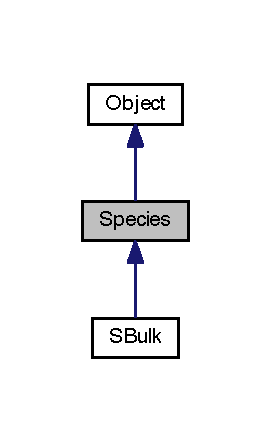
\includegraphics[width=350pt]{classSpecies__inherit__graph}
\end{center}
\end{figure}


Collaboration diagram for Species\+:\nopagebreak
\begin{figure}[H]
\begin{center}
\leavevmode
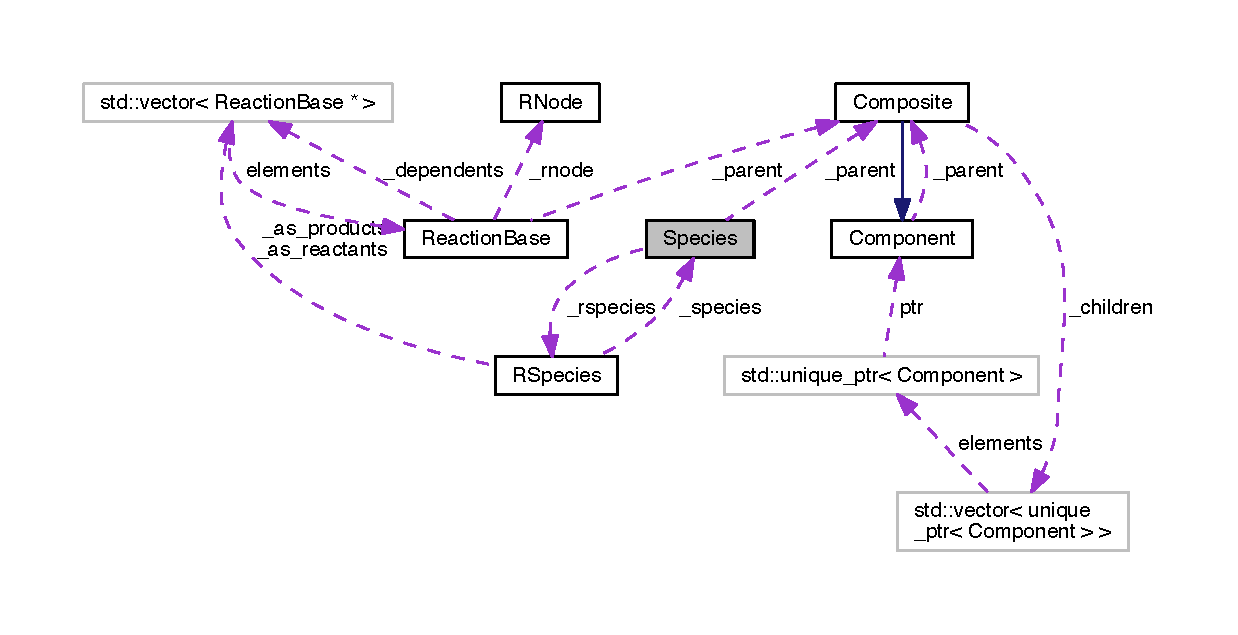
\includegraphics[width=350pt]{classSpecies__coll__graph}
\end{center}
\end{figure}
\subsection*{Public Member Functions}
\begin{DoxyCompactItemize}
\item 
\hyperlink{classSpecies_abb0f8e3208b0cc676157b7dff837c0be}{Species} ()
\begin{DoxyCompactList}\small\item\em Default Constructor; Should not be used by the end users -\/ only internally (although it is not marked as private) \end{DoxyCompactList}\item 
\hyperlink{classSpecies_a7c18ebc80eac720b2ee560a89587c13e}{Species} (const string \&name, \hyperlink{common_8h_a3503f321fd36304ee274141275cca586}{species\+\_\+copy\+\_\+t} n=0, \hyperlink{common_8h_a3503f321fd36304ee274141275cca586}{species\+\_\+copy\+\_\+t} ulim=\hyperlink{common_8h_adaf831a0b61083f29adf8fc6e8edab35}{max\+\_\+ulim})
\begin{DoxyCompactList}\small\item\em The constructor for this base class of \hyperlink{classSpecies}{Species} should not be called directly -\/ only by the concrete subclasses. \end{DoxyCompactList}\item 
\hyperlink{classSpecies_abfe20eea461a75aa2a5dce130480e9ce}{Species} (const \hyperlink{classSpecies}{Species} \&rhs)
\begin{DoxyCompactList}\small\item\em Copy constructor. \end{DoxyCompactList}\item 
\hyperlink{classSpecies_a0d8e3ec67f5d9d850237209763c46740}{Species} (\hyperlink{classSpecies}{Species} \&\&rhs) noexcept
\begin{DoxyCompactList}\small\item\em Move constructor -\/ makes it possible to easily add \hyperlink{classSpecies}{Species} to S\+T\+L containers, such as vector$<$\+Species$>$ One has to be careful with vector$<$\+Species$>$ as opposed to vector$<$\+Species$\ast$$>$. \end{DoxyCompactList}\item 
\hyperlink{classSpecies}{Species} \& \hyperlink{classSpecies_a0b0b78927bd86d5c46c6c58afd5fcf13}{operator=} (const \hyperlink{classSpecies}{Species} \&rhs)
\begin{DoxyCompactList}\small\item\em Assignment operator An assignment A = B copies the name of B to A. \end{DoxyCompactList}\item 
\hyperlink{classSpecies}{Species} \& \hyperlink{classSpecies_ac3f4cff8872442473bedcda82e5ef314}{operator=} (\hyperlink{classSpecies}{Species} \&\&rhs)
\begin{DoxyCompactList}\small\item\em Move assignment is needed for the same reasons as move constructor. \end{DoxyCompactList}\item 
virtual \hyperlink{classSpecies}{Species} $\ast$ \hyperlink{classSpecies_a5a7e96158d90d5f59f75c9e3405b54c6}{clone} ()
\item 
\hyperlink{classComposite}{Composite} $\ast$ \hyperlink{classSpecies_af24cab7cbaa561d35b08fef5faf05fdf}{get\+Parent} ()
\item 
void \hyperlink{classSpecies_acc64c5b61abf911872d433ac32b62de8}{set\+Parent} (\hyperlink{classComposite}{Composite} $\ast$other)
\item 
bool \hyperlink{classSpecies_a40262d7217fcc28a31682aee40a19232}{has\+Parent} () const 
\item 
\hyperlink{classComposite}{Composite} $\ast$ \hyperlink{classSpecies_a876c8a827476a11e05f3b7a7669c29b6}{get\+Root} ()
\item 
\hyperlink{classRSpecies}{R\+Species} \& \hyperlink{classSpecies_a048dd7bc3fecd08b1b1797dc83aa163d}{get\+R\+Species} ()
\begin{DoxyCompactList}\small\item\em Return a reference to \hyperlink{classRSpecies}{R\+Species}. \end{DoxyCompactList}\item 
const \hyperlink{classRSpecies}{R\+Species} \& \hyperlink{classSpecies_aa1069a34b360f84d186f48bd99f80971}{get\+R\+Species} () const 
\begin{DoxyCompactList}\small\item\em Return a constant reference to \hyperlink{classRSpecies}{R\+Species}. \end{DoxyCompactList}\item 
void \hyperlink{classSpecies_a88de7cf5130cb9cee2da3585374db654}{set\+N} (\hyperlink{common_8h_a3503f321fd36304ee274141275cca586}{species\+\_\+copy\+\_\+t} n)
\begin{DoxyCompactList}\small\item\em Sets the copy number for this \hyperlink{classSpecies}{Species}. \end{DoxyCompactList}\item 
\hyperlink{common_8h_a3503f321fd36304ee274141275cca586}{species\+\_\+copy\+\_\+t} \hyperlink{classSpecies_aea7327b3fed261c705b4d32b9973aa58}{get\+N} () const 
\begin{DoxyCompactList}\small\item\em Return the current copy number of this \hyperlink{classSpecies}{Species}. \end{DoxyCompactList}\item 
string \hyperlink{classSpecies_a28fa239dded841133760ff9c47af63a1}{get\+Name} () const 
\begin{DoxyCompactList}\small\item\em Return this \hyperlink{classSpecies}{Species}' name. \end{DoxyCompactList}\item 
int \hyperlink{classSpecies_a1ea8969c51bc69879891a408f9e197c7}{get\+Molecule} () const 
\begin{DoxyCompactList}\small\item\em Return the molecule index associated with this \hyperlink{classSpecies}{Species}' (as int) \end{DoxyCompactList}\item 
virtual \hyperlink{classSpecies_ac2c46c7a238233581e70685900dbb970}{$\sim$\+Species} () noexcept
\begin{DoxyCompactList}\small\item\em Virtual destructor. \end{DoxyCompactList}\item 
virtual string \hyperlink{classSpecies_a00dab56705525cefef915aa29363a959}{get\+Full\+Name} () const 
\begin{DoxyCompactList}\small\item\em Return the full name of this \hyperlink{classSpecies}{Species} in a string format (e.\+g. \char`\"{}\+Arp2/3\{\+Bulk\}\char`\"{}. \end{DoxyCompactList}\item 
virtual size\+\_\+t \hyperlink{classSpecies_a1864e111fe0304ca8d6b2d0d955a7356}{count\+Species} () const 
\end{DoxyCompactItemize}
\subsection*{Private Attributes}
\begin{DoxyCompactItemize}
\item 
int \hyperlink{classSpecies_a2cd51e66d421793bc3a8df9a7b0aa7d6}{\+\_\+molecule}
\begin{DoxyCompactList}\small\item\em unique id identifying the molecule (e.\+g. the integer id corresponding to \char`\"{}\+Arp2/3\char`\"{}) \end{DoxyCompactList}\item 
\hyperlink{classRSpecies}{R\+Species} $\ast$ \hyperlink{classSpecies_a8267607e66889feba64d1c00674337af}{\+\_\+rspecies}
\begin{DoxyCompactList}\small\item\em pointer to \hyperlink{classRSpecies}{R\+Species}; \hyperlink{classSpecies}{Species} is responsible for creating and destroying \hyperlink{classRSpecies}{R\+Species} \end{DoxyCompactList}\item 
\hyperlink{classComposite}{Composite} $\ast$ \hyperlink{classSpecies_a747392355a5d95f5dfd769a56076f538}{\+\_\+parent}
\begin{DoxyCompactList}\small\item\em pointer to the \char`\"{}container\char`\"{} object holding this \hyperlink{classSpecies}{Species} (could be a nullptr) \end{DoxyCompactList}\end{DoxyCompactItemize}
\subsection*{Friends}
\begin{DoxyCompactItemize}
\item 
bool \hyperlink{classSpecies_a22987c5719b74c50465256ea5b9d80bf}{operator==} (const \hyperlink{classSpecies}{Species} \&a, const \hyperlink{classSpecies}{Species} \&b)
\begin{DoxyCompactList}\small\item\em Returns true if two \hyperlink{classSpecies}{Species} objects are equal. \end{DoxyCompactList}\item 
bool \hyperlink{classSpecies_aff630d716711fbbab3bc7f598230316b}{operator!=} (const \hyperlink{classSpecies}{Species} \&a, const \hyperlink{classSpecies}{Species} \&b)
\begin{DoxyCompactList}\small\item\em Return true if two \hyperlink{classSpecies}{Species} are not equal. \end{DoxyCompactList}\end{DoxyCompactItemize}


\subsection{Detailed Description}
Represents chemical molecules, tracks their copy number and can be used in \hyperlink{classReaction}{Reactions}. 

This class represents chemical species, such as G-\/\+Actin. As a class, it provides \hyperlink{classSpecies}{Species}' name, the current copy number of molecules, \hyperlink{classSpecies}{Species} type (e.\+g. S\+Type\+::\+Bulk), and a few other characteristics of a \hyperlink{classSpecies}{Species}. This class is synergetic with the \hyperlink{classReaction}{Reaction}, since \hyperlink{classSpecies}{Species} can be added to \hyperlink{classReaction}{Reactions}.

As a type, \hyperlink{classSpecies}{Species} is composed of the following primary fields\+: type, name, copy number. A subclass may added additional primary fields. Two \hyperlink{classSpecies}{Species} are mathematically equal, if their primary fields are equal. This means that applying the copy constructor will guarantee that primary fields will be equal\+: 
\begin{DoxyCode}
\hyperlink{classSpeciesBulk}{SpeciesBulk} A\{\textcolor{stringliteral}{"Arp2/3"},25\};
\hyperlink{classSpeciesBulk}{SpeciesBulk} \hyperlink{namespaceA__B__C__Cycle_a9771d340c90ea87ee784c884fe2de3dc}{B}(A);
assert(A==\hyperlink{namespaceA__B__C__Cycle_a9771d340c90ea87ee784c884fe2de3dc}{B}); \textcolor{comment}{// A must be equal to B}
\end{DoxyCode}


\begin{DoxyNote}{Note}
Each \hyperlink{classSpecies}{Species} owns an unshared \hyperlink{classRSpecies}{R\+Species} object. However, the \hyperlink{classRSpecies}{R\+Species} field is not among the primary fields defining the \hyperlink{classSpecies}{Species} identity (hence, the equality operator). In particular, upon copying, the source and target \hyperlink{classSpecies}{Species} will have distinct \hyperlink{classRSpecies}{R\+Species} fields. However, in a fully constructed program, the source and target species (after applying the copy constructor) should eventually be involved in the same set of equivalent reactions. This means that their respective reactions will return true when the equlaity operator is applied.

The \hyperlink{classSpecies}{Species} class allows callbacks (see make\+Signaling and related methods). 
\end{DoxyNote}


Definition at line 128 of file Species.\+h.



\subsection{Constructor \& Destructor Documentation}
\hypertarget{classSpecies_abb0f8e3208b0cc676157b7dff837c0be}{\index{Species@{Species}!Species@{Species}}
\index{Species@{Species}!Species@{Species}}
\subsubsection[{Species}]{\setlength{\rightskip}{0pt plus 5cm}Species\+::\+Species (
\begin{DoxyParamCaption}
{}
\end{DoxyParamCaption}
)\hspace{0.3cm}{\ttfamily [inline]}}}\label{classSpecies_abb0f8e3208b0cc676157b7dff837c0be}


Default Constructor; Should not be used by the end users -\/ only internally (although it is not marked as private) 



Definition at line 135 of file Species.\+h.



References \+\_\+molecule, \+\_\+rspecies, Species\+Names\+D\+B\+::\+Instance(), and Species\+Names\+D\+B\+::string\+To\+Int().



Referenced by clone().

\hypertarget{classSpecies_a7c18ebc80eac720b2ee560a89587c13e}{\index{Species@{Species}!Species@{Species}}
\index{Species@{Species}!Species@{Species}}
\subsubsection[{Species}]{\setlength{\rightskip}{0pt plus 5cm}Species\+::\+Species (
\begin{DoxyParamCaption}
\item[{const string \&}]{name, }
\item[{{\bf species\+\_\+copy\+\_\+t}}]{n = {\ttfamily 0}, }
\item[{{\bf species\+\_\+copy\+\_\+t}}]{ulim = {\ttfamily {\bf max\+\_\+ulim}}}
\end{DoxyParamCaption}
)\hspace{0.3cm}{\ttfamily [inline]}}}\label{classSpecies_a7c18ebc80eac720b2ee560a89587c13e}


The constructor for this base class of \hyperlink{classSpecies}{Species} should not be called directly -\/ only by the concrete subclasses. 


\begin{DoxyParams}{Parameters}
{\em name} & -\/ a string for the \hyperlink{classSpecies}{Species} name associated with this \hyperlink{classSpecies}{Species}. For example, \char`\"{}\+G-\/\+Actin\char`\"{} or \char`\"{}\+Arp2/3\char`\"{} \\
\hline
{\em type\+\_\+enum} & -\/ S\+Type enum, such as S\+Type\+::\+Diffusing \\
\hline
{\em n} & -\/ copy number \\
\hline
{\em ulim} & -\/ upper limit for this species' copy number \\
\hline
\end{DoxyParams}


Definition at line 146 of file Species.\+h.



References \+\_\+molecule, \+\_\+rspecies, Species\+Names\+D\+B\+::\+Instance(), and Species\+Names\+D\+B\+::string\+To\+Int().

\hypertarget{classSpecies_abfe20eea461a75aa2a5dce130480e9ce}{\index{Species@{Species}!Species@{Species}}
\index{Species@{Species}!Species@{Species}}
\subsubsection[{Species}]{\setlength{\rightskip}{0pt plus 5cm}Species\+::\+Species (
\begin{DoxyParamCaption}
\item[{const {\bf Species} \&}]{rhs}
\end{DoxyParamCaption}
)\hspace{0.3cm}{\ttfamily [inline]}}}\label{classSpecies_abfe20eea461a75aa2a5dce130480e9ce}


Copy constructor. 

\begin{DoxyNote}{Note}
The associated \hyperlink{classRSpecies}{R\+Species} subpart is not copied, but a new one is created. This means that the copied destination \hyperlink{classSpecies}{Species} won't be included in any \hyperlink{classReaction}{Reaction} interactions of the original source \hyperlink{classSpecies}{Species}. The species copy numbered is copied to the target. The A \hyperlink{classSpecies}{Species} parent attriute is not copied, but set to nullptr. 
\end{DoxyNote}


Definition at line 158 of file Species.\+h.



References \+\_\+rspecies, and get\+N().

\hypertarget{classSpecies_a0d8e3ec67f5d9d850237209763c46740}{\index{Species@{Species}!Species@{Species}}
\index{Species@{Species}!Species@{Species}}
\subsubsection[{Species}]{\setlength{\rightskip}{0pt plus 5cm}Species\+::\+Species (
\begin{DoxyParamCaption}
\item[{{\bf Species} \&\&}]{rhs}
\end{DoxyParamCaption}
)\hspace{0.3cm}{\ttfamily [inline]}, {\ttfamily [noexcept]}}}\label{classSpecies_a0d8e3ec67f5d9d850237209763c46740}


Move constructor -\/ makes it possible to easily add \hyperlink{classSpecies}{Species} to S\+T\+L containers, such as vector$<$\+Species$>$ One has to be careful with vector$<$\+Species$>$ as opposed to vector$<$\+Species$\ast$$>$. 

The latter is \char`\"{}safe\char`\"{} in terms of being internally moved around by vector.\+resize, etc., but vector$<$\+Species$>$ would copy \hyperlink{classSpecies}{Species} if a move constructor is not available. This will then destruct the original \hyperlink{classSpecies}{Species} (with its associated \hyperlink{classRSpecies}{R\+Species}), hence, the \hyperlink{classReaction}{Reaction} network of the \hyperlink{classSpecies}{Species} will be lost. Since this behavior is most likely not desired or unacceptable, the internal vector operations should only \char`\"{}move\char`\"{} the \hyperlink{classSpecies}{Species} around, without copying. Moving transfers the \hyperlink{classRSpecies}{R\+Species} pointer from source to target, stealing resources from the source, leaving it for destruction. The \hyperlink{classSpecies}{Species} parent attriute is moved it. 

Definition at line 174 of file Species.\+h.

\hypertarget{classSpecies_ac2c46c7a238233581e70685900dbb970}{\index{Species@{Species}!````~Species@{$\sim$\+Species}}
\index{````~Species@{$\sim$\+Species}!Species@{Species}}
\subsubsection[{$\sim$\+Species}]{\setlength{\rightskip}{0pt plus 5cm}virtual Species\+::$\sim$\+Species (
\begin{DoxyParamCaption}
{}
\end{DoxyParamCaption}
)\hspace{0.3cm}{\ttfamily [inline]}, {\ttfamily [virtual]}, {\ttfamily [noexcept]}}}\label{classSpecies_ac2c46c7a238233581e70685900dbb970}


Virtual destructor. 

\begin{DoxyNote}{Note}
noexcept is important here. Otherwise, gcc flags the constructor as potentially throwing, which in turn disables move operations by the S\+T\+L containers. This behaviour is a gcc bug (as of gcc 4.\+703), and will presumbaly be fixed in the future. 
\end{DoxyNote}


Definition at line 286 of file Species.\+h.



References \+\_\+rspecies.



\subsection{Member Function Documentation}
\hypertarget{classSpecies_a5a7e96158d90d5f59f75c9e3405b54c6}{\index{Species@{Species}!clone@{clone}}
\index{clone@{clone}!Species@{Species}}
\subsubsection[{clone}]{\setlength{\rightskip}{0pt plus 5cm}virtual {\bf Species}$\ast$ Species\+::clone (
\begin{DoxyParamCaption}
{}
\end{DoxyParamCaption}
)\hspace{0.3cm}{\ttfamily [inline]}, {\ttfamily [virtual]}}}\label{classSpecies_a5a7e96158d90d5f59f75c9e3405b54c6}


Reimplemented in \hyperlink{classSpeciesMinusEnd_a21083383e254146fd074161c7b2cf88b}{Species\+Minus\+End}, \hyperlink{classSpeciesPlusEnd_a359b23c2ec95d9ead3f8f40d1bc641de}{Species\+Plus\+End}, \hyperlink{classSpeciesMotor_a8b035f81717d4c29546f47ada9924b62}{Species\+Motor}, \hyperlink{classSpeciesLinker_a5555ddb310465ae43ec89927236d2fc8}{Species\+Linker}, \hyperlink{classSpeciesBound_a729e4ef2724698f48c45e17972fa1726}{Species\+Bound}, \hyperlink{classSpeciesFilament_a1a4b86c27795ca658c65ac415f8861a7}{Species\+Filament}, \hyperlink{classSpeciesDiffusing_af3b8326e4b81d2bb4d65630ee7a49995}{Species\+Diffusing}, and \hyperlink{classSpeciesBulk_a4bca7120d95d6303f66a5bca30a2612b}{Species\+Bulk}.



Definition at line 205 of file Species.\+h.



References Species().

\hypertarget{classSpecies_a1864e111fe0304ca8d6b2d0d955a7356}{\index{Species@{Species}!count\+Species@{count\+Species}}
\index{count\+Species@{count\+Species}!Species@{Species}}
\subsubsection[{count\+Species}]{\setlength{\rightskip}{0pt plus 5cm}virtual size\+\_\+t Species\+::count\+Species (
\begin{DoxyParamCaption}
{}
\end{DoxyParamCaption}
) const\hspace{0.3cm}{\ttfamily [inline]}, {\ttfamily [virtual]}}}\label{classSpecies_a1864e111fe0304ca8d6b2d0d955a7356}


Definition at line 295 of file Species.\+h.

\hypertarget{classSpecies_a00dab56705525cefef915aa29363a959}{\index{Species@{Species}!get\+Full\+Name@{get\+Full\+Name}}
\index{get\+Full\+Name@{get\+Full\+Name}!Species@{Species}}
\subsubsection[{get\+Full\+Name}]{\setlength{\rightskip}{0pt plus 5cm}virtual string Species\+::get\+Full\+Name (
\begin{DoxyParamCaption}
{}
\end{DoxyParamCaption}
) const\hspace{0.3cm}{\ttfamily [inline]}, {\ttfamily [virtual]}}}\label{classSpecies_a00dab56705525cefef915aa29363a959}


Return the full name of this \hyperlink{classSpecies}{Species} in a string format (e.\+g. \char`\"{}\+Arp2/3\{\+Bulk\}\char`\"{}. 



Reimplemented in \hyperlink{classSpeciesMinusEnd_a0c22b4471bd9ca01b2795838e5d4e46a}{Species\+Minus\+End}, \hyperlink{classSpeciesPlusEnd_aa010e7adb578155bf0142fa84684b47e}{Species\+Plus\+End}, \hyperlink{classSpeciesMotor_a31f9c0c447c007c1ba04bb0ce1d9c0e1}{Species\+Motor}, \hyperlink{classSpeciesLinker_a4f964e32cd7d13d86ea75cb962511f3a}{Species\+Linker}, \hyperlink{classSpeciesBound_a251dcc12a2599a4df36155539cb0efeb}{Species\+Bound}, \hyperlink{classSpeciesFilament_a18ee4cfa2eb8ba642b97996924564292}{Species\+Filament}, \hyperlink{classSpeciesDiffusing_a143bb7cf1e7dfbd4d514224b4d0ba042}{Species\+Diffusing}, and \hyperlink{classSpeciesBulk_aeb3983d890dae341fe53355c4b29dc6b}{Species\+Bulk}.



Definition at line 293 of file Species.\+h.



References get\+Name().



Referenced by R\+Species\+::get\+Full\+Name(), and operator$<$$<$().

\hypertarget{classSpecies_a1ea8969c51bc69879891a408f9e197c7}{\index{Species@{Species}!get\+Molecule@{get\+Molecule}}
\index{get\+Molecule@{get\+Molecule}!Species@{Species}}
\subsubsection[{get\+Molecule}]{\setlength{\rightskip}{0pt plus 5cm}int Species\+::get\+Molecule (
\begin{DoxyParamCaption}
{}
\end{DoxyParamCaption}
) const\hspace{0.3cm}{\ttfamily [inline]}}}\label{classSpecies_a1ea8969c51bc69879891a408f9e197c7}


Return the molecule index associated with this \hyperlink{classSpecies}{Species}' (as int) 



Definition at line 241 of file Species.\+h.



References \+\_\+molecule.



Referenced by Compartment\+::add\+Species\+Bound(), Compartment\+::add\+Species\+Diffusing(), Compartment\+::add\+Species\+Filament(), Compartment\+::add\+Species\+Linker(), Compartment\+::add\+Species\+Minus\+End(), Compartment\+::add\+Species\+Motor(), Compartment\+::add\+Species\+Plus\+End(), Compartment\+::add\+Species\+Unique(), and Compartment\+::set\+Diffusion\+Rate().

\hypertarget{classSpecies_aea7327b3fed261c705b4d32b9973aa58}{\index{Species@{Species}!get\+N@{get\+N}}
\index{get\+N@{get\+N}!Species@{Species}}
\subsubsection[{get\+N}]{\setlength{\rightskip}{0pt plus 5cm}{\bf species\+\_\+copy\+\_\+t} Species\+::get\+N (
\begin{DoxyParamCaption}
{}
\end{DoxyParamCaption}
) const\hspace{0.3cm}{\ttfamily [inline]}}}\label{classSpecies_aea7327b3fed261c705b4d32b9973aa58}


Return the current copy number of this \hyperlink{classSpecies}{Species}. 



Definition at line 230 of file Species.\+h.



References \+\_\+rspecies, and R\+Species\+::get\+N().



Referenced by Linker\+::\+Linker(), main(), Motor\+Ghost\+::\+Motor\+Ghost(), operator$<$$<$(), operator=(), C\+Monomer\+::print(), Species(), Linker\+::$\sim$\+Linker(), and Motor\+Ghost\+::$\sim$\+Motor\+Ghost().

\hypertarget{classSpecies_a28fa239dded841133760ff9c47af63a1}{\index{Species@{Species}!get\+Name@{get\+Name}}
\index{get\+Name@{get\+Name}!Species@{Species}}
\subsubsection[{get\+Name}]{\setlength{\rightskip}{0pt plus 5cm}string Species\+::get\+Name (
\begin{DoxyParamCaption}
{}
\end{DoxyParamCaption}
) const\hspace{0.3cm}{\ttfamily [inline]}}}\label{classSpecies_a28fa239dded841133760ff9c47af63a1}


Return this \hyperlink{classSpecies}{Species}' name. 



Definition at line 238 of file Species.\+h.



References \+\_\+molecule, Species\+Names\+D\+B\+::\+Instance(), and Species\+Names\+D\+B\+::int\+To\+String().



Referenced by get\+Full\+Name(), Species\+Bulk\+::get\+Full\+Name(), Species\+Diffusing\+::get\+Full\+Name(), Species\+Filament\+::get\+Full\+Name(), Species\+Bound\+::get\+Full\+Name(), Species\+Linker\+::get\+Full\+Name(), Species\+Motor\+::get\+Full\+Name(), Species\+Plus\+End\+::get\+Full\+Name(), Species\+Minus\+End\+::get\+Full\+Name(), and C\+Monomer\+::print().

\hypertarget{classSpecies_af24cab7cbaa561d35b08fef5faf05fdf}{\index{Species@{Species}!get\+Parent@{get\+Parent}}
\index{get\+Parent@{get\+Parent}!Species@{Species}}
\subsubsection[{get\+Parent}]{\setlength{\rightskip}{0pt plus 5cm}{\bf Composite}$\ast$ Species\+::get\+Parent (
\begin{DoxyParamCaption}
{}
\end{DoxyParamCaption}
)\hspace{0.3cm}{\ttfamily [inline]}}}\label{classSpecies_af24cab7cbaa561d35b08fef5faf05fdf}


Definition at line 209 of file Species.\+h.



References \+\_\+parent.



Referenced by get\+Root(), and main().

\hypertarget{classSpecies_a876c8a827476a11e05f3b7a7669c29b6}{\index{Species@{Species}!get\+Root@{get\+Root}}
\index{get\+Root@{get\+Root}!Species@{Species}}
\subsubsection[{get\+Root}]{\setlength{\rightskip}{0pt plus 5cm}{\bf Composite} $\ast$ Species\+::get\+Root (
\begin{DoxyParamCaption}
{}
\end{DoxyParamCaption}
)}}\label{classSpecies_a876c8a827476a11e05f3b7a7669c29b6}


Definition at line 36 of file Species.\+cpp.



References get\+Parent(), Component\+::get\+Root(), and has\+Parent().

\hypertarget{classSpecies_a048dd7bc3fecd08b1b1797dc83aa163d}{\index{Species@{Species}!get\+R\+Species@{get\+R\+Species}}
\index{get\+R\+Species@{get\+R\+Species}!Species@{Species}}
\subsubsection[{get\+R\+Species}]{\setlength{\rightskip}{0pt plus 5cm}{\bf R\+Species}\& Species\+::get\+R\+Species (
\begin{DoxyParamCaption}
{}
\end{DoxyParamCaption}
)\hspace{0.3cm}{\ttfamily [inline]}}}\label{classSpecies_a048dd7bc3fecd08b1b1797dc83aa163d}


Return a reference to \hyperlink{classRSpecies}{R\+Species}. 

Notice that value copying won't be allowed because \hyperlink{classRSpecies}{R\+Species} is not copyable. 

Definition at line 219 of file Species.\+h.



References \+\_\+rspecies.



Referenced by Chem\+Signal\+::connect(), Simple\+Manager\+Impl\+::initialize\+C\+Cylinder(), Linker\+::\+Linker(), main(), Motor\+Ghost\+::\+Motor\+Ghost(), Linker\+::$\sim$\+Linker(), and Motor\+Ghost\+::$\sim$\+Motor\+Ghost().

\hypertarget{classSpecies_aa1069a34b360f84d186f48bd99f80971}{\index{Species@{Species}!get\+R\+Species@{get\+R\+Species}}
\index{get\+R\+Species@{get\+R\+Species}!Species@{Species}}
\subsubsection[{get\+R\+Species}]{\setlength{\rightskip}{0pt plus 5cm}const {\bf R\+Species}\& Species\+::get\+R\+Species (
\begin{DoxyParamCaption}
{}
\end{DoxyParamCaption}
) const\hspace{0.3cm}{\ttfamily [inline]}}}\label{classSpecies_aa1069a34b360f84d186f48bd99f80971}


Return a constant reference to \hyperlink{classRSpecies}{R\+Species}. 



Definition at line 222 of file Species.\+h.



References \+\_\+rspecies.

\hypertarget{classSpecies_a40262d7217fcc28a31682aee40a19232}{\index{Species@{Species}!has\+Parent@{has\+Parent}}
\index{has\+Parent@{has\+Parent}!Species@{Species}}
\subsubsection[{has\+Parent}]{\setlength{\rightskip}{0pt plus 5cm}bool Species\+::has\+Parent (
\begin{DoxyParamCaption}
{}
\end{DoxyParamCaption}
) const\hspace{0.3cm}{\ttfamily [inline]}}}\label{classSpecies_a40262d7217fcc28a31682aee40a19232}


Definition at line 213 of file Species.\+h.



References \+\_\+parent.



Referenced by get\+Root().

\hypertarget{classSpecies_a0b0b78927bd86d5c46c6c58afd5fcf13}{\index{Species@{Species}!operator=@{operator=}}
\index{operator=@{operator=}!Species@{Species}}
\subsubsection[{operator=}]{\setlength{\rightskip}{0pt plus 5cm}{\bf Species}\& Species\+::operator= (
\begin{DoxyParamCaption}
\item[{const {\bf Species} \&}]{rhs}
\end{DoxyParamCaption}
)\hspace{0.3cm}{\ttfamily [inline]}}}\label{classSpecies_a0b0b78927bd86d5c46c6c58afd5fcf13}


Assignment operator An assignment A = B copies the name of B to A. 

It destroys the \hyperlink{classReaction}{Reaction} interactions of A, and resents them to a blank value (i.\+e. A won't be involced in any Reactions). B's \hyperlink{classReaction}{Reaction} interactions are not copied. The copy number of B is copied to A. The A \hyperlink{classSpecies}{Species} parent attriute is not copied, but set to nullptr. 

Definition at line 183 of file Species.\+h.



References \+\_\+molecule, \+\_\+parent, \+\_\+rspecies, and get\+N().



Referenced by Species\+Bulk\+::operator=(), Species\+Diffusing\+::operator=(), Species\+Filament\+::operator=(), Species\+Bound\+::operator=(), Species\+Plus\+End\+::operator=(), and Species\+Minus\+End\+::operator=().

\hypertarget{classSpecies_ac3f4cff8872442473bedcda82e5ef314}{\index{Species@{Species}!operator=@{operator=}}
\index{operator=@{operator=}!Species@{Species}}
\subsubsection[{operator=}]{\setlength{\rightskip}{0pt plus 5cm}{\bf Species}\& Species\+::operator= (
\begin{DoxyParamCaption}
\item[{{\bf Species} \&\&}]{rhs}
\end{DoxyParamCaption}
)\hspace{0.3cm}{\ttfamily [inline]}}}\label{classSpecies_ac3f4cff8872442473bedcda82e5ef314}


Move assignment is needed for the same reasons as move constructor. 

\begin{DoxySeeAlso}{See also}
\hyperlink{classSpecies}{Species} (\hyperlink{classSpecies}{Species} \&\&rhs) 
\end{DoxySeeAlso}


Definition at line 197 of file Species.\+h.



References \+\_\+molecule, \+\_\+parent, and \+\_\+rspecies.

\hypertarget{classSpecies_a88de7cf5130cb9cee2da3585374db654}{\index{Species@{Species}!set\+N@{set\+N}}
\index{set\+N@{set\+N}!Species@{Species}}
\subsubsection[{set\+N}]{\setlength{\rightskip}{0pt plus 5cm}void Species\+::set\+N (
\begin{DoxyParamCaption}
\item[{{\bf species\+\_\+copy\+\_\+t}}]{n}
\end{DoxyParamCaption}
)\hspace{0.3cm}{\ttfamily [inline]}}}\label{classSpecies_a88de7cf5130cb9cee2da3585374db654}


Sets the copy number for this \hyperlink{classSpecies}{Species}. 


\begin{DoxyParams}{Parameters}
{\em n} & should be a non-\/negative number, but no checking is done in run time \\
\hline
\end{DoxyParams}
\begin{DoxyNote}{Note}
The operation does not emit any signals about the copy number change. 
\end{DoxyNote}


Definition at line 227 of file Species.\+h.



References \+\_\+rspecies, and R\+Species\+::set\+N().

\hypertarget{classSpecies_acc64c5b61abf911872d433ac32b62de8}{\index{Species@{Species}!set\+Parent@{set\+Parent}}
\index{set\+Parent@{set\+Parent}!Species@{Species}}
\subsubsection[{set\+Parent}]{\setlength{\rightskip}{0pt plus 5cm}void Species\+::set\+Parent (
\begin{DoxyParamCaption}
\item[{{\bf Composite} $\ast$}]{other}
\end{DoxyParamCaption}
)\hspace{0.3cm}{\ttfamily [inline]}}}\label{classSpecies_acc64c5b61abf911872d433ac32b62de8}


Definition at line 211 of file Species.\+h.



References \+\_\+parent.



Referenced by Compartment\+::add\+Species\+Bound(), Compartment\+::add\+Species\+Diffusing(), Compartment\+::add\+Species\+Filament(), Compartment\+::add\+Species\+Linker(), Compartment\+::add\+Species\+Minus\+End(), Compartment\+::add\+Species\+Motor(), Compartment\+::add\+Species\+Plus\+End(), and Compartment\+::add\+Species\+Unique().



\subsection{Friends And Related Function Documentation}
\hypertarget{classSpecies_aff630d716711fbbab3bc7f598230316b}{\index{Species@{Species}!operator"!=@{operator"!=}}
\index{operator"!=@{operator"!=}!Species@{Species}}
\subsubsection[{operator"!=}]{\setlength{\rightskip}{0pt plus 5cm}bool operator!= (
\begin{DoxyParamCaption}
\item[{const {\bf Species} \&}]{a, }
\item[{const {\bf Species} \&}]{b}
\end{DoxyParamCaption}
)\hspace{0.3cm}{\ttfamily [friend]}}}\label{classSpecies_aff630d716711fbbab3bc7f598230316b}


Return true if two \hyperlink{classSpecies}{Species} are not equal. 

\begin{DoxySeeAlso}{See also}
\hyperlink{classSpecies_a22987c5719b74c50465256ea5b9d80bf}{operator ==(const Species\& a, const Species\& b)} above 
\end{DoxySeeAlso}


Definition at line 276 of file Species.\+h.

\hypertarget{classSpecies_a22987c5719b74c50465256ea5b9d80bf}{\index{Species@{Species}!operator==@{operator==}}
\index{operator==@{operator==}!Species@{Species}}
\subsubsection[{operator==}]{\setlength{\rightskip}{0pt plus 5cm}bool operator== (
\begin{DoxyParamCaption}
\item[{const {\bf Species} \&}]{a, }
\item[{const {\bf Species} \&}]{b}
\end{DoxyParamCaption}
)\hspace{0.3cm}{\ttfamily [friend]}}}\label{classSpecies_a22987c5719b74c50465256ea5b9d80bf}


Returns true if two \hyperlink{classSpecies}{Species} objects are equal. 

This function would accept derived class of \hyperlink{classSpecies}{Species}, such as \hyperlink{classSpeciesBulk}{Species\+Bulk} Two \hyperlink{classSpecies}{Species} are equal if their S\+Type(s) are equal (i.\+e. are of the same class), their names are equal. 

Definition at line 267 of file Species.\+h.



\subsection{Member Data Documentation}
\hypertarget{classSpecies_a2cd51e66d421793bc3a8df9a7b0aa7d6}{\index{Species@{Species}!\+\_\+molecule@{\+\_\+molecule}}
\index{\+\_\+molecule@{\+\_\+molecule}!Species@{Species}}
\subsubsection[{\+\_\+molecule}]{\setlength{\rightskip}{0pt plus 5cm}int Species\+::\+\_\+molecule\hspace{0.3cm}{\ttfamily [private]}}}\label{classSpecies_a2cd51e66d421793bc3a8df9a7b0aa7d6}


unique id identifying the molecule (e.\+g. the integer id corresponding to \char`\"{}\+Arp2/3\char`\"{}) 



Definition at line 130 of file Species.\+h.



Referenced by get\+Molecule(), get\+Name(), operator=(), and Species().

\hypertarget{classSpecies_a747392355a5d95f5dfd769a56076f538}{\index{Species@{Species}!\+\_\+parent@{\+\_\+parent}}
\index{\+\_\+parent@{\+\_\+parent}!Species@{Species}}
\subsubsection[{\+\_\+parent}]{\setlength{\rightskip}{0pt plus 5cm}{\bf Composite}$\ast$ Species\+::\+\_\+parent\hspace{0.3cm}{\ttfamily [private]}}}\label{classSpecies_a747392355a5d95f5dfd769a56076f538}


pointer to the \char`\"{}container\char`\"{} object holding this \hyperlink{classSpecies}{Species} (could be a nullptr) 



Definition at line 132 of file Species.\+h.



Referenced by get\+Parent(), has\+Parent(), operator=(), and set\+Parent().

\hypertarget{classSpecies_a8267607e66889feba64d1c00674337af}{\index{Species@{Species}!\+\_\+rspecies@{\+\_\+rspecies}}
\index{\+\_\+rspecies@{\+\_\+rspecies}!Species@{Species}}
\subsubsection[{\+\_\+rspecies}]{\setlength{\rightskip}{0pt plus 5cm}{\bf R\+Species}$\ast$ Species\+::\+\_\+rspecies\hspace{0.3cm}{\ttfamily [private]}}}\label{classSpecies_a8267607e66889feba64d1c00674337af}


pointer to \hyperlink{classRSpecies}{R\+Species}; \hyperlink{classSpecies}{Species} is responsible for creating and destroying \hyperlink{classRSpecies}{R\+Species} 



Definition at line 131 of file Species.\+h.



Referenced by get\+N(), get\+R\+Species(), operator=(), set\+N(), Species(), and $\sim$\+Species().



The documentation for this class was generated from the following files\+:\begin{DoxyCompactItemize}
\item 
M3\+S\+Y\+M/\+Structure/\hyperlink{Species_8h}{Species.\+h}\item 
M3\+S\+Y\+M/\+Structure/\hyperlink{Species_8cpp}{Species.\+cpp}\end{DoxyCompactItemize}

\hypertarget{structspecies__type__tag}{\section{species\-\_\-type\-\_\-tag Struct Reference}
\label{structspecies__type__tag}\index{species\-\_\-type\-\_\-tag@{species\-\_\-type\-\_\-tag}}
}


Create a tag for the corresponding Species\-Type flywheights.  




{\ttfamily \#include $<$Species.\-h$>$}



\subsection{Detailed Description}
Create a tag for the corresponding Species\-Type flywheights. 

Definition at line 31 of file Species.\-h.



The documentation for this struct was generated from the following file\-:\begin{DoxyCompactItemize}
\item 
/\-Users/papoian/\-Dropbox/\-Codes/\-Cyto\-Sim/\-Cyto\-Sim/\hyperlink{Species_8h}{Species.\-h}\end{DoxyCompactItemize}

\hypertarget{classSpeciesDB}{\section{Species\-D\-B Class Reference}
\label{classSpeciesDB}\index{Species\-D\-B@{Species\-D\-B}}
}


\hyperlink{classSpeciesDB}{Species\-D\-B} should be used for obtaining new objects of the \hyperlink{classSpecies}{Species} hieararchy.  




{\ttfamily \#include $<$Species\-D\-B.\-h$>$}

\subsection*{Public Member Functions}
\begin{DoxyCompactItemize}
\item 
void \hyperlink{classSpeciesDB_a8c6c7e5c59cf237210b4f91c4235f165}{Initialize} ()
\item 
\hyperlink{classSpecies}{Species} $\ast$ \hyperlink{classSpeciesDB_ace46d47499b147c9cb17c18d06e8558a}{make\-Species} (const \hyperlink{Species_8h_af8f3afcc030f67a124aa4a6b5badf495}{Species\-Type} \&name, int N=0)
\item 
\hyperlink{classSBulk}{S\-Bulk} $\ast$ \hyperlink{classSpeciesDB_a0cb94a600f33c10032595e8fc008c969}{make\-S\-Bulk} (const \hyperlink{Species_8h_af8f3afcc030f67a124aa4a6b5badf495}{Species\-Type} \&name, int N=0)
\end{DoxyCompactItemize}
\subsection*{Static Public Member Functions}
\begin{DoxyCompactItemize}
\item 
static \hyperlink{classSpeciesDB}{Species\-D\-B} $\ast$ \hyperlink{classSpeciesDB_a8f3e30d93fd019bf0d0d0f657a81794f}{get\-Instance} ()
\end{DoxyCompactItemize}


\subsection{Detailed Description}
\hyperlink{classSpeciesDB}{Species\-D\-B} should be used for obtaining new objects of the \hyperlink{classSpecies}{Species} hieararchy. 

It internally uses the Standard\-Species\-Factory to accomplish the construction. It is also a database that can be queried to obtain a pointer to a \hyperlink{classSpecies}{Species} if the \hyperlink{classSpecies}{Species}' I\-D is known. This class is a singleton, and should be used like this\-: 
\begin{DoxyCode}
 SpeciesDB *sdb = SpeciesDB::getInstance();
 sdb->Initialize();
\end{DoxyCode}
 

Definition at line 38 of file Species\-D\-B.\-h.



\subsection{Member Function Documentation}
\hypertarget{classSpeciesDB_a8f3e30d93fd019bf0d0d0f657a81794f}{\index{Species\-D\-B@{Species\-D\-B}!get\-Instance@{get\-Instance}}
\index{get\-Instance@{get\-Instance}!SpeciesDB@{Species\-D\-B}}
\subsubsection[{get\-Instance}]{\setlength{\rightskip}{0pt plus 5cm}{\bf Species\-D\-B} $\ast$ {\bf Species\-D\-B\-::get\-Instance} (
\begin{DoxyParamCaption}
{}
\end{DoxyParamCaption}
)\hspace{0.3cm}{\ttfamily  \mbox{[}static\mbox{]}}}}\label{classSpeciesDB_a8f3e30d93fd019bf0d0d0f657a81794f}


Definition at line 14 of file Species\-D\-B.\-cpp.



Referenced by main().

\hypertarget{classSpeciesDB_a8c6c7e5c59cf237210b4f91c4235f165}{\index{Species\-D\-B@{Species\-D\-B}!Initialize@{Initialize}}
\index{Initialize@{Initialize}!SpeciesDB@{Species\-D\-B}}
\subsubsection[{Initialize}]{\setlength{\rightskip}{0pt plus 5cm}void {\bf Species\-D\-B\-::\-Initialize} (
\begin{DoxyParamCaption}
{}
\end{DoxyParamCaption}
)}}\label{classSpeciesDB_a8c6c7e5c59cf237210b4f91c4235f165}


Definition at line 21 of file Species\-D\-B.\-cpp.



Referenced by main().

\hypertarget{classSpeciesDB_a0cb94a600f33c10032595e8fc008c969}{\index{Species\-D\-B@{Species\-D\-B}!make\-S\-Bulk@{make\-S\-Bulk}}
\index{make\-S\-Bulk@{make\-S\-Bulk}!SpeciesDB@{Species\-D\-B}}
\subsubsection[{make\-S\-Bulk}]{\setlength{\rightskip}{0pt plus 5cm}{\bf S\-Bulk}$\ast$ {\bf Species\-D\-B\-::make\-S\-Bulk} (
\begin{DoxyParamCaption}
\item[{const {\bf Species\-Type} \&}]{name, }
\item[{int}]{N = {\ttfamily 0}}
\end{DoxyParamCaption}
)\hspace{0.3cm}{\ttfamily  \mbox{[}inline\mbox{]}}}}\label{classSpeciesDB_a0cb94a600f33c10032595e8fc008c969}


Definition at line 47 of file Species\-D\-B.\-h.



References Species\-Factory\-::make\-S\-Bulk().



Referenced by main().

\hypertarget{classSpeciesDB_ace46d47499b147c9cb17c18d06e8558a}{\index{Species\-D\-B@{Species\-D\-B}!make\-Species@{make\-Species}}
\index{make\-Species@{make\-Species}!SpeciesDB@{Species\-D\-B}}
\subsubsection[{make\-Species}]{\setlength{\rightskip}{0pt plus 5cm}{\bf Species}$\ast$ {\bf Species\-D\-B\-::make\-Species} (
\begin{DoxyParamCaption}
\item[{const {\bf Species\-Type} \&}]{name, }
\item[{int}]{N = {\ttfamily 0}}
\end{DoxyParamCaption}
)\hspace{0.3cm}{\ttfamily  \mbox{[}inline\mbox{]}}}}\label{classSpeciesDB_ace46d47499b147c9cb17c18d06e8558a}


Definition at line 42 of file Species\-D\-B.\-h.



References Species\-Factory\-::make\-Species().



Referenced by main().



The documentation for this class was generated from the following files\-:\begin{DoxyCompactItemize}
\item 
/\-Users/papoian/\-Dropbox/\-Codes/\-Cyto\-Sim/\-Cyto\-Sim/\hyperlink{SpeciesDB_8h}{Species\-D\-B.\-h}\item 
/\-Users/papoian/\-Dropbox/\-Codes/\-Cyto\-Sim/\-Cyto\-Sim/\hyperlink{SpeciesDB_8cpp}{Species\-D\-B.\-cpp}\end{DoxyCompactItemize}

\hypertarget{classSpeciesFactory}{\section{Species\-Factory Class Reference}
\label{classSpeciesFactory}\index{Species\-Factory@{Species\-Factory}}
}


{\ttfamily \#include $<$Species.\-h$>$}



\subsection{Detailed Description}


Definition at line 77 of file Species.\-h.



The documentation for this class was generated from the following file\-:\begin{DoxyCompactItemize}
\item 
Cyto\-Sim/\hyperlink{Species_8h}{Species.\-h}\end{DoxyCompactItemize}

\chapter{File Documentation}
\hypertarget{common_8h}{\section{Cyto\-Sim/common.h File Reference}
\label{common_8h}\index{Cyto\-Sim/common.\-h@{Cyto\-Sim/common.\-h}}
}
{\ttfamily \#include $<$cstdint$>$}\\*
Include dependency graph for common.\-h\-:\nopagebreak
\begin{figure}[H]
\begin{center}
\leavevmode
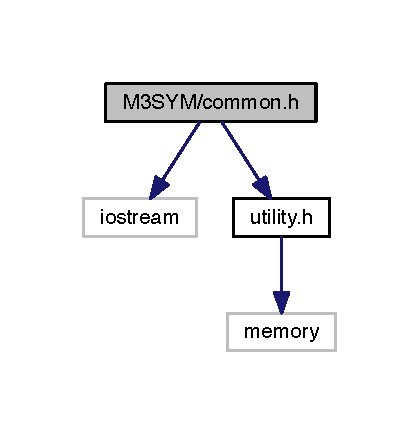
\includegraphics[width=178pt]{common_8h__incl}
\end{center}
\end{figure}
This graph shows which files directly or indirectly include this file\-:\nopagebreak
\begin{figure}[H]
\begin{center}
\leavevmode
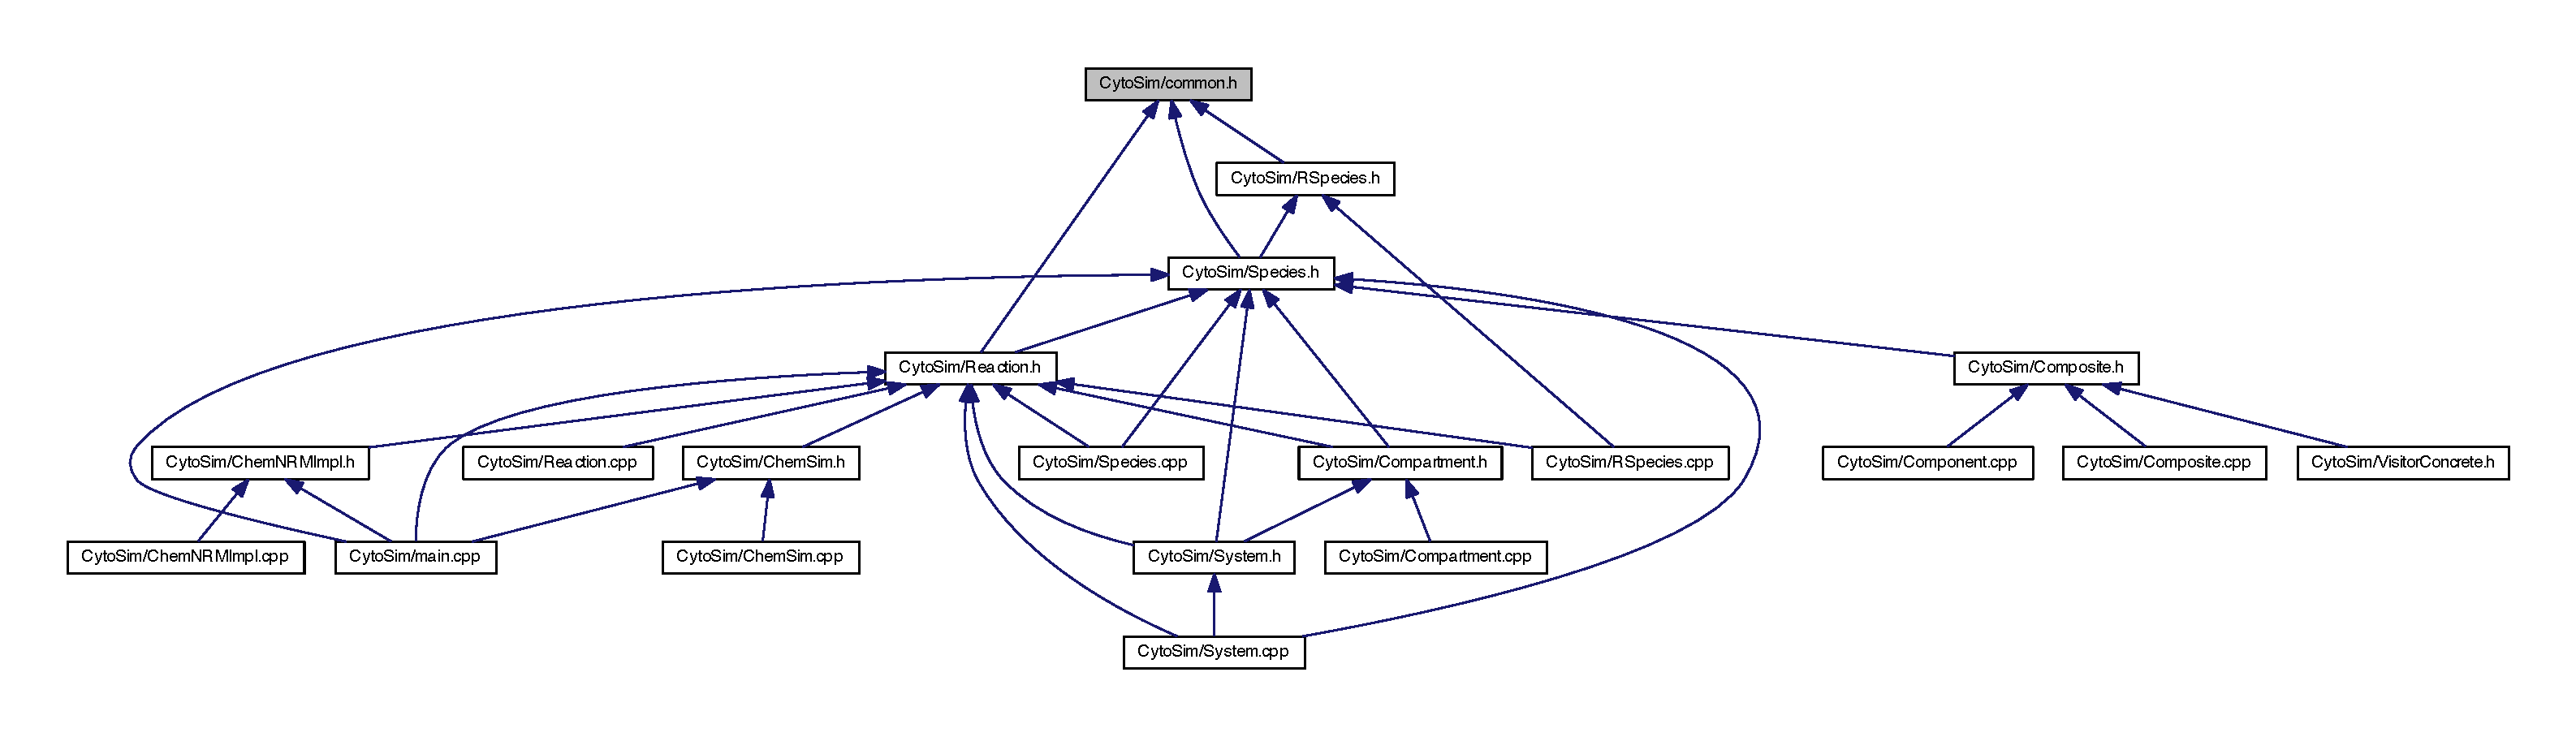
\includegraphics[width=350pt]{common_8h__dep__incl}
\end{center}
\end{figure}
\subsection*{Defines}
\begin{DoxyCompactItemize}
\item 
\#define \hyperlink{common_8h_ac331c2ee4410c5495c7d06314fdbc888}{T\-R\-A\-C\-K\-\_\-\-D\-E\-P\-E\-N\-D\-E\-N\-T\-S}
\item 
\#define \hyperlink{common_8h_a03fd44bcbf25c32054a4982f84f45259}{T\-R\-A\-C\-K\-\_\-\-Z\-E\-R\-O\-\_\-\-C\-O\-P\-Y\-\_\-\-N}
\item 
\#define \hyperlink{common_8h_a318b9661d7fcfe101415b83880576138}{T\-R\-A\-C\-K\-\_\-\-U\-P\-P\-E\-R\-\_\-\-C\-O\-P\-Y\-\_\-\-N}
\end{DoxyCompactItemize}
\subsection*{Typedefs}
\begin{DoxyCompactItemize}
\item 
typedef unsigned short \hyperlink{common_8h_a3503f321fd36304ee274141275cca586}{species\-\_\-copy\-\_\-t}
\end{DoxyCompactItemize}
\subsection*{Functions}
\begin{DoxyCompactItemize}
\item 
double \hyperlink{common_8h_abca55e6a21e0401c42bfb5da79ad3ad5}{tau} ()
\end{DoxyCompactItemize}
\subsection*{Variables}
\begin{DoxyCompactItemize}
\item 
const \hyperlink{common_8h_a3503f321fd36304ee274141275cca586}{species\-\_\-copy\-\_\-t} \hyperlink{common_8h_adaf831a0b61083f29adf8fc6e8edab35}{max\-\_\-ulim} = 1024
\item 
double \hyperlink{common_8h_aa3ea98c7e5ad42511b3ec7e0e90e61a4}{global\-\_\-time}
\end{DoxyCompactItemize}


\subsection{Define Documentation}
\hypertarget{common_8h_ac331c2ee4410c5495c7d06314fdbc888}{\index{common.\-h@{common.\-h}!T\-R\-A\-C\-K\-\_\-\-D\-E\-P\-E\-N\-D\-E\-N\-T\-S@{T\-R\-A\-C\-K\-\_\-\-D\-E\-P\-E\-N\-D\-E\-N\-T\-S}}
\index{T\-R\-A\-C\-K\-\_\-\-D\-E\-P\-E\-N\-D\-E\-N\-T\-S@{T\-R\-A\-C\-K\-\_\-\-D\-E\-P\-E\-N\-D\-E\-N\-T\-S}!common.h@{common.\-h}}
\subsubsection[{T\-R\-A\-C\-K\-\_\-\-D\-E\-P\-E\-N\-D\-E\-N\-T\-S}]{\setlength{\rightskip}{0pt plus 5cm}\#define {\bf T\-R\-A\-C\-K\-\_\-\-D\-E\-P\-E\-N\-D\-E\-N\-T\-S}}}\label{common_8h_ac331c2ee4410c5495c7d06314fdbc888}


Definition at line 12 of file common.\-h.

\hypertarget{common_8h_a318b9661d7fcfe101415b83880576138}{\index{common.\-h@{common.\-h}!T\-R\-A\-C\-K\-\_\-\-U\-P\-P\-E\-R\-\_\-\-C\-O\-P\-Y\-\_\-\-N@{T\-R\-A\-C\-K\-\_\-\-U\-P\-P\-E\-R\-\_\-\-C\-O\-P\-Y\-\_\-\-N}}
\index{T\-R\-A\-C\-K\-\_\-\-U\-P\-P\-E\-R\-\_\-\-C\-O\-P\-Y\-\_\-\-N@{T\-R\-A\-C\-K\-\_\-\-U\-P\-P\-E\-R\-\_\-\-C\-O\-P\-Y\-\_\-\-N}!common.h@{common.\-h}}
\subsubsection[{T\-R\-A\-C\-K\-\_\-\-U\-P\-P\-E\-R\-\_\-\-C\-O\-P\-Y\-\_\-\-N}]{\setlength{\rightskip}{0pt plus 5cm}\#define {\bf T\-R\-A\-C\-K\-\_\-\-U\-P\-P\-E\-R\-\_\-\-C\-O\-P\-Y\-\_\-\-N}}}\label{common_8h_a318b9661d7fcfe101415b83880576138}


Definition at line 14 of file common.\-h.

\hypertarget{common_8h_a03fd44bcbf25c32054a4982f84f45259}{\index{common.\-h@{common.\-h}!T\-R\-A\-C\-K\-\_\-\-Z\-E\-R\-O\-\_\-\-C\-O\-P\-Y\-\_\-\-N@{T\-R\-A\-C\-K\-\_\-\-Z\-E\-R\-O\-\_\-\-C\-O\-P\-Y\-\_\-\-N}}
\index{T\-R\-A\-C\-K\-\_\-\-Z\-E\-R\-O\-\_\-\-C\-O\-P\-Y\-\_\-\-N@{T\-R\-A\-C\-K\-\_\-\-Z\-E\-R\-O\-\_\-\-C\-O\-P\-Y\-\_\-\-N}!common.h@{common.\-h}}
\subsubsection[{T\-R\-A\-C\-K\-\_\-\-Z\-E\-R\-O\-\_\-\-C\-O\-P\-Y\-\_\-\-N}]{\setlength{\rightskip}{0pt plus 5cm}\#define {\bf T\-R\-A\-C\-K\-\_\-\-Z\-E\-R\-O\-\_\-\-C\-O\-P\-Y\-\_\-\-N}}}\label{common_8h_a03fd44bcbf25c32054a4982f84f45259}


Definition at line 13 of file common.\-h.



\subsection{Typedef Documentation}
\hypertarget{common_8h_a3503f321fd36304ee274141275cca586}{\index{common.\-h@{common.\-h}!species\-\_\-copy\-\_\-t@{species\-\_\-copy\-\_\-t}}
\index{species\-\_\-copy\-\_\-t@{species\-\_\-copy\-\_\-t}!common.h@{common.\-h}}
\subsubsection[{species\-\_\-copy\-\_\-t}]{\setlength{\rightskip}{0pt plus 5cm}typedef unsigned short {\bf species\-\_\-copy\-\_\-t}}}\label{common_8h_a3503f321fd36304ee274141275cca586}


Definition at line 18 of file common.\-h.



\subsection{Function Documentation}
\hypertarget{common_8h_abca55e6a21e0401c42bfb5da79ad3ad5}{\index{common.\-h@{common.\-h}!tau@{tau}}
\index{tau@{tau}!common.h@{common.\-h}}
\subsubsection[{tau}]{\setlength{\rightskip}{0pt plus 5cm}double {\bf tau} (
\begin{DoxyParamCaption}
{}
\end{DoxyParamCaption}
)\hspace{0.3cm}{\ttfamily  \mbox{[}inline\mbox{]}}}}\label{common_8h_abca55e6a21e0401c42bfb5da79ad3ad5}


Definition at line 22 of file common.\-h.



References global\-\_\-time.



Referenced by chem\-::\-R\-Node\-N\-R\-M\-::generate\-New\-Rand\-Tau(), chem\-::\-Chem\-Simple\-Gillespie\-Impl\-::make\-Step(), chem\-::\-Chem\-Gillespie\-Impl\-::make\-Step(), chem\-::\-R\-Node\-N\-R\-M\-::passivate\-Reaction(), and chem\-::\-R\-Node\-N\-R\-M\-::set\-Tau().



\subsection{Variable Documentation}
\hypertarget{common_8h_aa3ea98c7e5ad42511b3ec7e0e90e61a4}{\index{common.\-h@{common.\-h}!global\-\_\-time@{global\-\_\-time}}
\index{global\-\_\-time@{global\-\_\-time}!common.h@{common.\-h}}
\subsubsection[{global\-\_\-time}]{\setlength{\rightskip}{0pt plus 5cm}double {\bf global\-\_\-time}}}\label{common_8h_aa3ea98c7e5ad42511b3ec7e0e90e61a4}


Definition at line 11 of file common.\-cpp.



Referenced by chem\-::\-Chem\-Simple\-Gillespie\-Impl\-::sync\-Global\-Time(), chem\-::\-Chem\-Gillespie\-Impl\-::sync\-Global\-Time(), chem\-::\-Chem\-N\-R\-M\-Impl\-::sync\-Global\-Time(), and tau().

\hypertarget{common_8h_adaf831a0b61083f29adf8fc6e8edab35}{\index{common.\-h@{common.\-h}!max\-\_\-ulim@{max\-\_\-ulim}}
\index{max\-\_\-ulim@{max\-\_\-ulim}!common.h@{common.\-h}}
\subsubsection[{max\-\_\-ulim}]{\setlength{\rightskip}{0pt plus 5cm}const {\bf species\-\_\-copy\-\_\-t} {\bf max\-\_\-ulim} = 1024}}\label{common_8h_adaf831a0b61083f29adf8fc6e8edab35}


Definition at line 19 of file common.\-h.


\hypertarget{main_8cpp}{\section{Cyto\-Sim/main.cpp File Reference}
\label{main_8cpp}\index{Cyto\-Sim/main.\-cpp@{Cyto\-Sim/main.\-cpp}}
}
{\ttfamily \#include $<$iostream$>$}\\*
{\ttfamily \#include $<$fstream$>$}\\*
{\ttfamily \#include \char`\"{}Species\-D\-B.\-h\char`\"{}}\\*
Include dependency graph for main.\-cpp\-:
\nopagebreak
\begin{figure}[H]
\begin{center}
\leavevmode
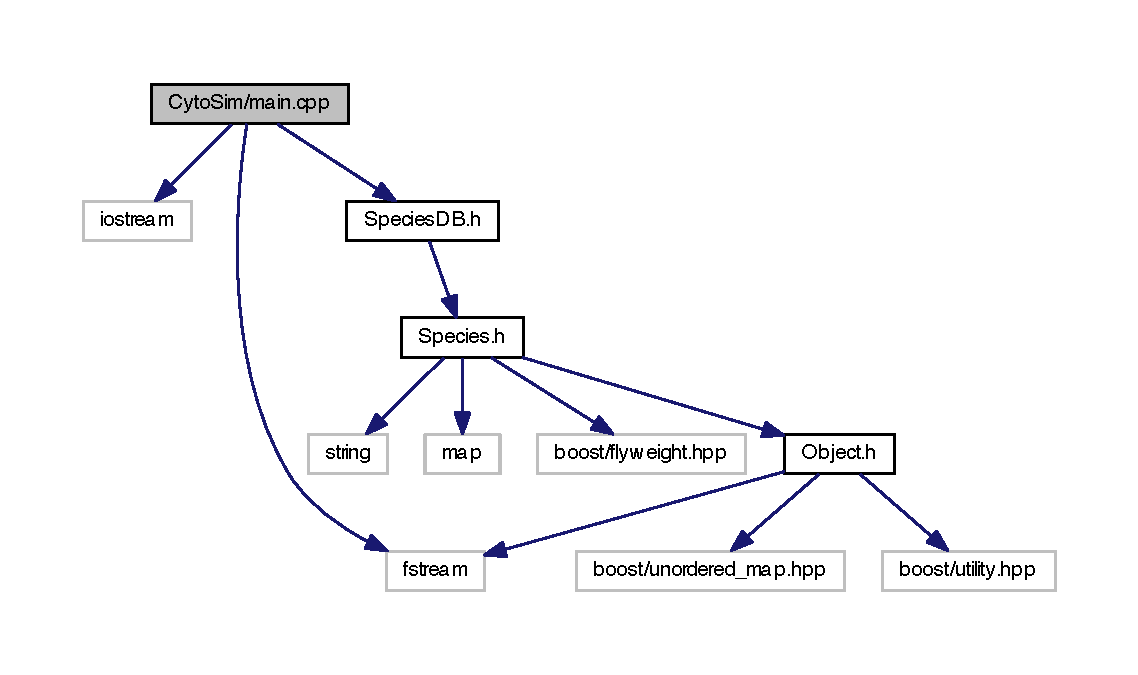
\includegraphics[width=350pt]{main_8cpp__incl}
\end{center}
\end{figure}
\subsection*{Functions}
\begin{DoxyCompactItemize}
\item 
int \hyperlink{main_8cpp_ac0f2228420376f4db7e1274f2b41667c}{main} (int argc, const char $\ast$argv\mbox{[}$\,$\mbox{]})
\end{DoxyCompactItemize}


\subsection{Function Documentation}
\hypertarget{main_8cpp_ac0f2228420376f4db7e1274f2b41667c}{\index{main.\-cpp@{main.\-cpp}!main@{main}}
\index{main@{main}!main.cpp@{main.\-cpp}}
\subsubsection[{main}]{\setlength{\rightskip}{0pt plus 5cm}int {\bf main} (
\begin{DoxyParamCaption}
\item[{int}]{argc, }
\item[{const char $\ast$}]{argv\mbox{[}$\,$\mbox{]}}
\end{DoxyParamCaption}
)}}\label{main_8cpp_ac0f2228420376f4db7e1274f2b41667c}


Definition at line 38 of file main.\-cpp.



References Species\-D\-B\-::get\-Instance(), Species\-D\-B\-::\-Initialize(), Species\-D\-B\-::make\-S\-Bulk(), Species\-D\-B\-::make\-Species(), Species\-::write\-Self(), and S\-Bulk\-::write\-Self().


\hypertarget{Object_8cpp}{\section{/\-Users/papoian/\-Dropbox/\-Codes/\-Cyto\-Sim/\-Cyto\-Sim/\-Object.cpp File Reference}
\label{Object_8cpp}\index{/\-Users/papoian/\-Dropbox/\-Codes/\-Cyto\-Sim/\-Cyto\-Sim/\-Object.\-cpp@{/\-Users/papoian/\-Dropbox/\-Codes/\-Cyto\-Sim/\-Cyto\-Sim/\-Object.\-cpp}}
}
{\ttfamily \#include \char`\"{}Object.\-h\char`\"{}}\\*
{\ttfamily \#include $<$assert.\-h$>$}\\*
Include dependency graph for Object.\-cpp\-:\nopagebreak
\begin{figure}[H]
\begin{center}
\leavevmode
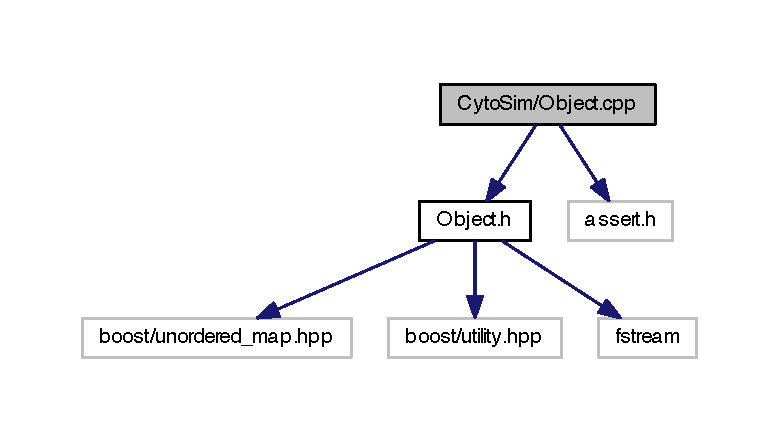
\includegraphics[width=350pt]{Object_8cpp__incl}
\end{center}
\end{figure}

\hypertarget{Object_8h}{\section{/\-Users/papoian/\-Dropbox/\-Codes/\-Cyto\-Sim/\-Cyto\-Sim/\-Object.h File Reference}
\label{Object_8h}\index{/\-Users/papoian/\-Dropbox/\-Codes/\-Cyto\-Sim/\-Cyto\-Sim/\-Object.\-h@{/\-Users/papoian/\-Dropbox/\-Codes/\-Cyto\-Sim/\-Cyto\-Sim/\-Object.\-h}}
}


this header file will contain defininition of class \hyperlink{classObject}{Object} and related classes and methods $\ast$  


{\ttfamily \#include $<$boost/unordered\-\_\-map.\-hpp$>$}\\*
{\ttfamily \#include $<$boost/utility.\-hpp$>$}\\*
{\ttfamily \#include $<$fstream$>$}\\*
Include dependency graph for Object.\-h\-:\nopagebreak
\begin{figure}[H]
\begin{center}
\leavevmode
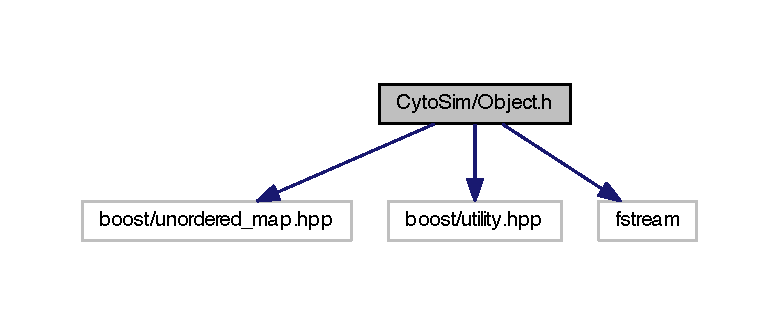
\includegraphics[width=350pt]{Object_8h__incl}
\end{center}
\end{figure}
This graph shows which files directly or indirectly include this file\-:\nopagebreak
\begin{figure}[H]
\begin{center}
\leavevmode
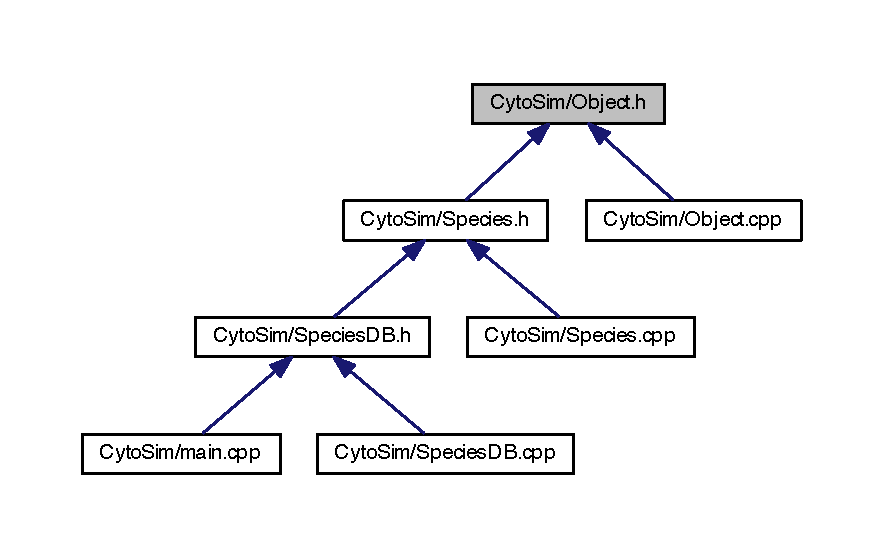
\includegraphics[width=350pt]{Object_8h__dep__incl}
\end{center}
\end{figure}
\subsection*{Classes}
\begin{DoxyCompactItemize}
\item 
class \hyperlink{classObject}{Object}
\end{DoxyCompactItemize}
\subsection*{Typedefs}
\begin{DoxyCompactItemize}
\item 
typedef unsigned long \hyperlink{Object_8h_a0b56ddf6ace42572542aae1f2c364e05}{object\-\_\-id}
\begin{DoxyCompactList}\small\item\em object\-\_\-id is the type used for the P\-R\-I\-M\-A\-R\-Y K\-E\-Y of the \hyperlink{classObject}{Object} database \end{DoxyCompactList}\item 
typedef boost\-::unordered\-\_\-map\\*
$<$ \hyperlink{Object_8h_a0b56ddf6ace42572542aae1f2c364e05}{object\-\_\-id}, \hyperlink{classObject}{Object} $\ast$ $>$ \hyperlink{Object_8h_a2c8fbe32166b1ac6c99f427ef9632332}{Map\-I\-D\-Obj\-Ptr}
\end{DoxyCompactItemize}


\subsection{Detailed Description}
this header file will contain defininition of class \hyperlink{classObject}{Object} and related classes and methods $\ast$ \begin{DoxyAuthor}{Author}
Garegin Papoian $\ast$ 
\end{DoxyAuthor}
\begin{DoxyDate}{Date}
4/8/2012 
\end{DoxyDate}


Definition in file \hyperlink{Object_8h_source}{Object.\-h}.



\subsection{Typedef Documentation}
\hypertarget{Object_8h_a2c8fbe32166b1ac6c99f427ef9632332}{\index{Object.\-h@{Object.\-h}!Map\-I\-D\-Obj\-Ptr@{Map\-I\-D\-Obj\-Ptr}}
\index{Map\-I\-D\-Obj\-Ptr@{Map\-I\-D\-Obj\-Ptr}!Object.h@{Object.\-h}}
\subsubsection[{Map\-I\-D\-Obj\-Ptr}]{\setlength{\rightskip}{0pt plus 5cm}typedef boost\-::unordered\-\_\-map$<${\bf object\-\_\-id}, {\bf Object} $\ast$$>$ {\bf Map\-I\-D\-Obj\-Ptr}}}\label{Object_8h_a2c8fbe32166b1ac6c99f427ef9632332}


Definition at line 30 of file Object.\-h.

\hypertarget{Object_8h_a0b56ddf6ace42572542aae1f2c364e05}{\index{Object.\-h@{Object.\-h}!object\-\_\-id@{object\-\_\-id}}
\index{object\-\_\-id@{object\-\_\-id}!Object.h@{Object.\-h}}
\subsubsection[{object\-\_\-id}]{\setlength{\rightskip}{0pt plus 5cm}typedef unsigned long {\bf object\-\_\-id}}}\label{Object_8h_a0b56ddf6ace42572542aae1f2c364e05}


object\-\_\-id is the type used for the P\-R\-I\-M\-A\-R\-Y K\-E\-Y of the \hyperlink{classObject}{Object} database 



Definition at line 25 of file Object.\-h.


\hypertarget{Species_8cpp}{\section{M3\+S\+Y\+M/\+Structure/\+Species.cpp File Reference}
\label{Species_8cpp}\index{M3\+S\+Y\+M/\+Structure/\+Species.\+cpp@{M3\+S\+Y\+M/\+Structure/\+Species.\+cpp}}
}
{\ttfamily \#include \char`\"{}Species.\+h\char`\"{}}\\*
{\ttfamily \#include \char`\"{}Reaction.\+h\char`\"{}}\\*
{\ttfamily \#include \char`\"{}Composite.\+h\char`\"{}}\\*
Include dependency graph for Species.\+cpp\+:\nopagebreak
\begin{figure}[H]
\begin{center}
\leavevmode
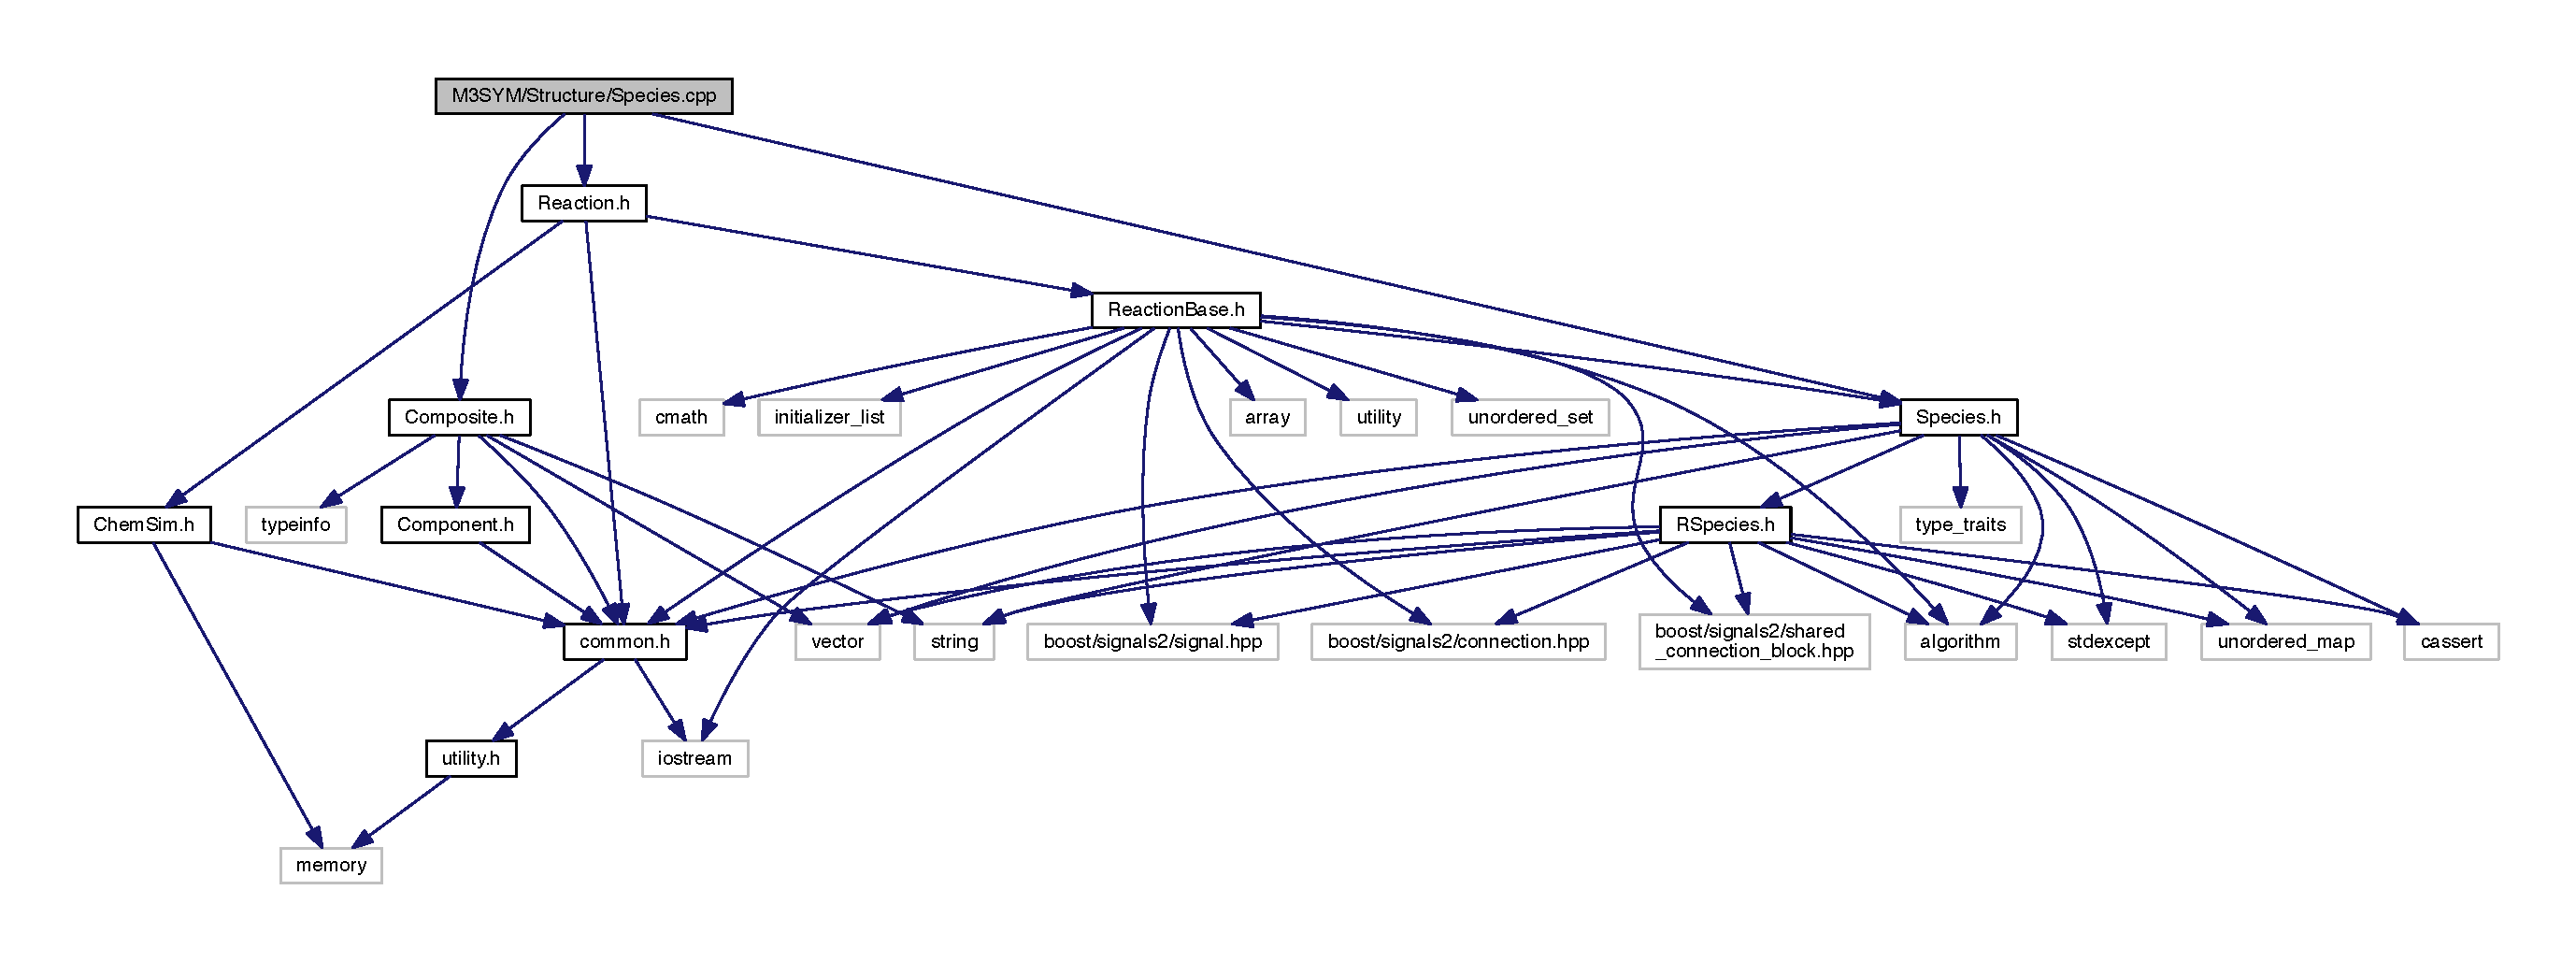
\includegraphics[width=350pt]{Species_8cpp__incl}
\end{center}
\end{figure}
\subsection*{Functions}
\begin{DoxyCompactItemize}
\item 
ostream \& \hyperlink{Species_8cpp_a4816bb7d9ee0557b45580bb9ece06e0d}{operator$<$$<$} (ostream \&os, const \hyperlink{classSpecies}{Species} \&s)
\begin{DoxyCompactList}\small\item\em Print self into an iostream. \end{DoxyCompactList}\end{DoxyCompactItemize}


\subsection{Function Documentation}
\hypertarget{Species_8cpp_a4816bb7d9ee0557b45580bb9ece06e0d}{\index{Species.\+cpp@{Species.\+cpp}!operator$<$$<$@{operator$<$$<$}}
\index{operator$<$$<$@{operator$<$$<$}!Species.\+cpp@{Species.\+cpp}}
\subsubsection[{operator$<$$<$}]{\setlength{\rightskip}{0pt plus 5cm}ostream\& operator$<$$<$ (
\begin{DoxyParamCaption}
\item[{ostream \&}]{os, }
\item[{const {\bf Species} \&}]{s}
\end{DoxyParamCaption}
)}}\label{Species_8cpp_a4816bb7d9ee0557b45580bb9ece06e0d}


Print self into an iostream. 



Definition at line 43 of file Species.\+cpp.



References Species\+::get\+Full\+Name(), and Species\+::get\+N().


\hypertarget{Species_8h}{\section{Cyto\-Sim/\-Species.h File Reference}
\label{Species_8h}\index{Cyto\-Sim/\-Species.\-h@{Cyto\-Sim/\-Species.\-h}}
}


this header file will contain defininition of the Species hieararchy and associated D\-B and helper classes.  


{\ttfamily \#include $<$vector$>$}\\*
{\ttfamily \#include $<$string$>$}\\*
{\ttfamily \#include $<$unordered\-\_\-map$>$}\\*
{\ttfamily \#include $<$algorithm$>$}\\*
{\ttfamily \#include $<$cassert$>$}\\*
{\ttfamily \#include $<$stdexcept$>$}\\*
{\ttfamily \#include $<$type\-\_\-traits$>$}\\*
{\ttfamily \#include \char`\"{}common.\-h\char`\"{}}\\*
{\ttfamily \#include \char`\"{}utility.\-h\char`\"{}}\\*
{\ttfamily \#include \char`\"{}Component.\-h\char`\"{}}\\*
{\ttfamily \#include \char`\"{}R\-Species.\-h\char`\"{}}\\*
Include dependency graph for Species.\-h\-:\nopagebreak
\begin{figure}[H]
\begin{center}
\leavevmode
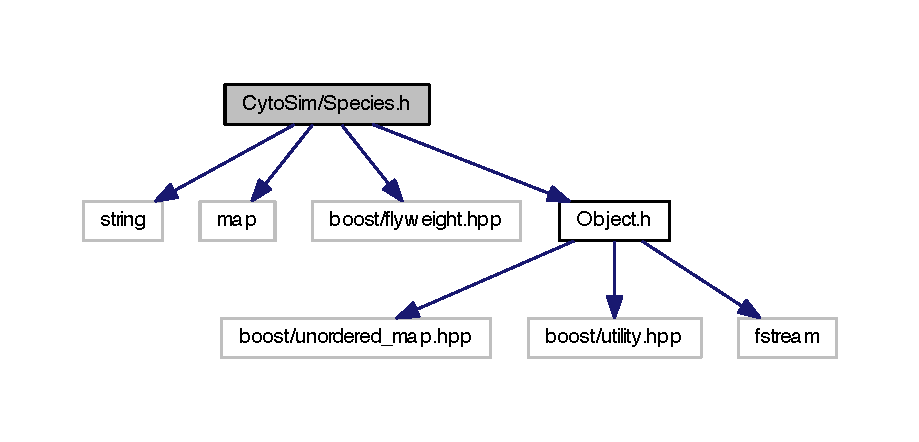
\includegraphics[width=350pt]{Species_8h__incl}
\end{center}
\end{figure}
This graph shows which files directly or indirectly include this file\-:\nopagebreak
\begin{figure}[H]
\begin{center}
\leavevmode
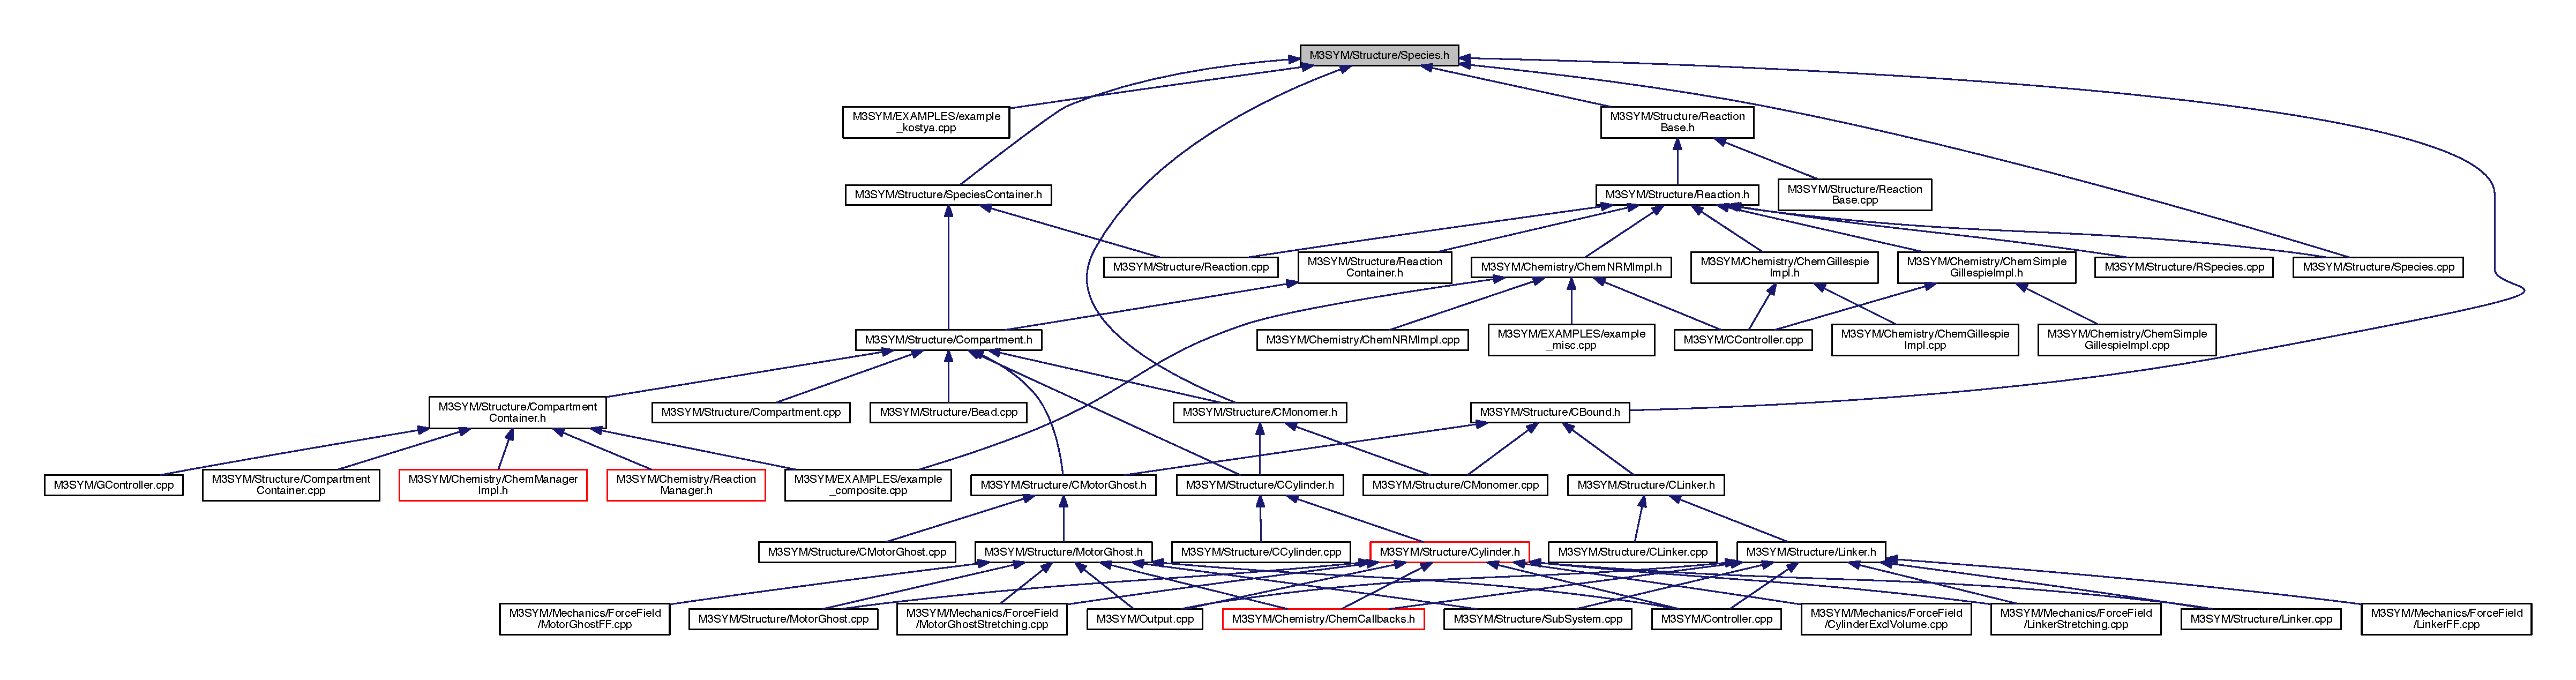
\includegraphics[width=350pt]{Species_8h__dep__incl}
\end{center}
\end{figure}
\subsection*{Classes}
\begin{DoxyCompactItemize}
\item 
class \hyperlink{classchem_1_1SpeciesNamesDB}{chem\-::\-Species\-Names\-D\-B}
\begin{DoxyCompactList}\small\item\em \hyperlink{classchem_1_1SpeciesNamesDB}{Species\-Names\-D\-B} class is used to associate unique integers with character based names of \hyperlink{classchem_1_1Species}{Species}. \end{DoxyCompactList}\item 
class \hyperlink{classchem_1_1Species}{chem\-::\-Species}
\begin{DoxyCompactList}\small\item\em \hyperlink{classchem_1_1Species}{Species} class represents chemical molecules, tracks their copy number and can be used in \hyperlink{classchem_1_1Reaction}{Reactions}. \end{DoxyCompactList}\item 
class \hyperlink{classchem_1_1SpeciesBulk}{chem\-::\-Species\-Bulk}
\begin{DoxyCompactList}\small\item\em \hyperlink{classchem_1_1SpeciesBulk}{Species\-Bulk} should be used for \hyperlink{classchem_1_1Species}{Species} without spatial information (i.\-e. well-\/mixed in the container) \end{DoxyCompactList}\item 
class \hyperlink{classchem_1_1SpeciesDiffusing}{chem\-::\-Species\-Diffusing}
\begin{DoxyCompactList}\small\item\em \hyperlink{classchem_1_1SpeciesDiffusing}{Species\-Diffusing} should be used for \hyperlink{classchem_1_1Species}{Species} which can move spatially from one compartment to the neighboring one (i.\-e. they are the stochastic analogue of determenistic reaction-\/diffusion processes) \end{DoxyCompactList}\end{DoxyCompactItemize}
\subsection*{Namespaces}
\begin{DoxyCompactItemize}
\item 
namespace \hyperlink{namespacechem}{chem}
\begin{DoxyCompactList}\small\item\em The algorithm implemented here is based on the following reference\-: $\ast$$\ast$ Michael A. Gibson, and Jehoshua Bruck J. Phys. Chem. A, 2000, 104 (9), 1876-\/1889 $\ast$$\ast$. \end{DoxyCompactList}\end{DoxyCompactItemize}
\subsection*{Functions}
\begin{DoxyCompactItemize}
\item 
std\-::ostream \& \hyperlink{Species_8h_a7b999c6dd7df6ab3481749c5d0bbe4fa}{operator$<$$<$} (std\-::ostream \&os, const \hyperlink{classchem_1_1Species}{chem\-::\-Species} \&s)
\begin{DoxyCompactList}\small\item\em Print self into an iostream. \end{DoxyCompactList}\end{DoxyCompactItemize}


\subsection{Detailed Description}
this header file will contain defininition of the Species hieararchy and associated D\-B and helper classes. \begin{DoxyAuthor}{Author}
Garegin Papoian $\ast$ 
\end{DoxyAuthor}
\begin{DoxyDate}{Date}
5/12/2012 
\end{DoxyDate}


Definition in file \hyperlink{Species_8h_source}{Species.\-h}.



\subsection{Function Documentation}
\hypertarget{Species_8h_a7b999c6dd7df6ab3481749c5d0bbe4fa}{\index{Species.\-h@{Species.\-h}!operator$<$$<$@{operator$<$$<$}}
\index{operator$<$$<$@{operator$<$$<$}!Species.h@{Species.\-h}}
\subsubsection[{operator$<$$<$}]{\setlength{\rightskip}{0pt plus 5cm}std\-::ostream\& operator$<$$<$ (
\begin{DoxyParamCaption}
\item[{std\-::ostream \&}]{os, }
\item[{const {\bf chem\-::\-Species} \&}]{s}
\end{DoxyParamCaption}
)}}\label{Species_8h_a7b999c6dd7df6ab3481749c5d0bbe4fa}


Print self into an iostream. 



Definition at line 51 of file Species.\-cpp.



References chem\-::\-Species\-::get\-Full\-Name(), and chem\-::\-Species\-::get\-N().


\hypertarget{SpeciesDB_8cpp}{\section{/\-Users/papoian/\-Dropbox/\-Codes/\-Cyto\-Sim/\-Cyto\-Sim/\-Species\-D\-B.cpp File Reference}
\label{SpeciesDB_8cpp}\index{/\-Users/papoian/\-Dropbox/\-Codes/\-Cyto\-Sim/\-Cyto\-Sim/\-Species\-D\-B.\-cpp@{/\-Users/papoian/\-Dropbox/\-Codes/\-Cyto\-Sim/\-Cyto\-Sim/\-Species\-D\-B.\-cpp}}
}
{\ttfamily \#include $<$iostream$>$}\\*
{\ttfamily \#include \char`\"{}Species\-D\-B.\-h\char`\"{}}\\*
Include dependency graph for Species\-D\-B.\-cpp\-:\nopagebreak
\begin{figure}[H]
\begin{center}
\leavevmode
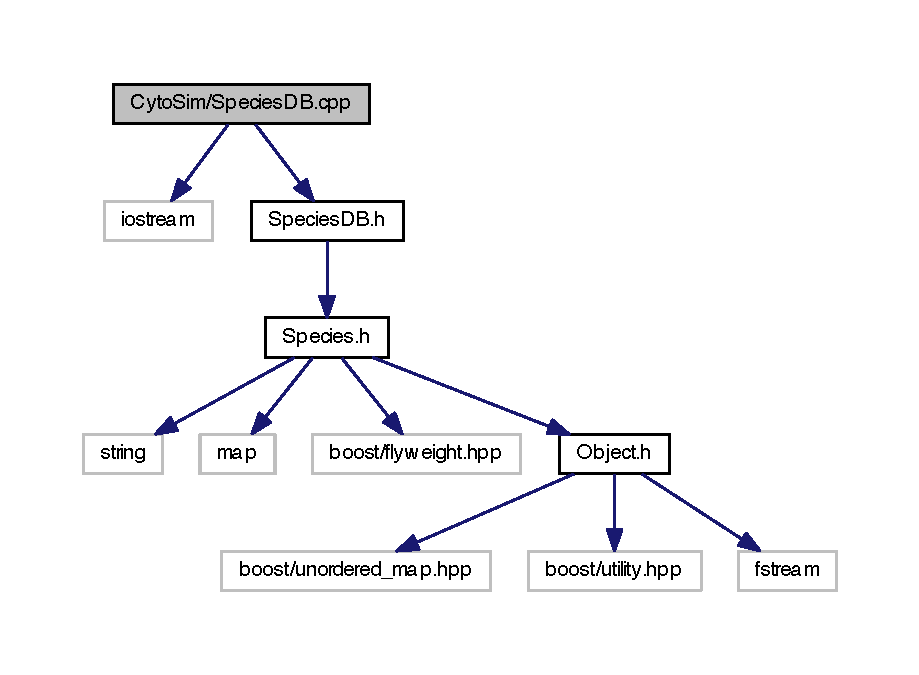
\includegraphics[width=350pt]{SpeciesDB_8cpp__incl}
\end{center}
\end{figure}

\hypertarget{SpeciesDB_8h}{\section{Cyto\-Sim/\-Species\-D\-B.h File Reference}
\label{SpeciesDB_8h}\index{Cyto\-Sim/\-Species\-D\-B.\-h@{Cyto\-Sim/\-Species\-D\-B.\-h}}
}
{\ttfamily \#include \char`\"{}Species.\-h\char`\"{}}\\*
Include dependency graph for Species\-D\-B.\-h\-:
\nopagebreak
\begin{figure}[H]
\begin{center}
\leavevmode
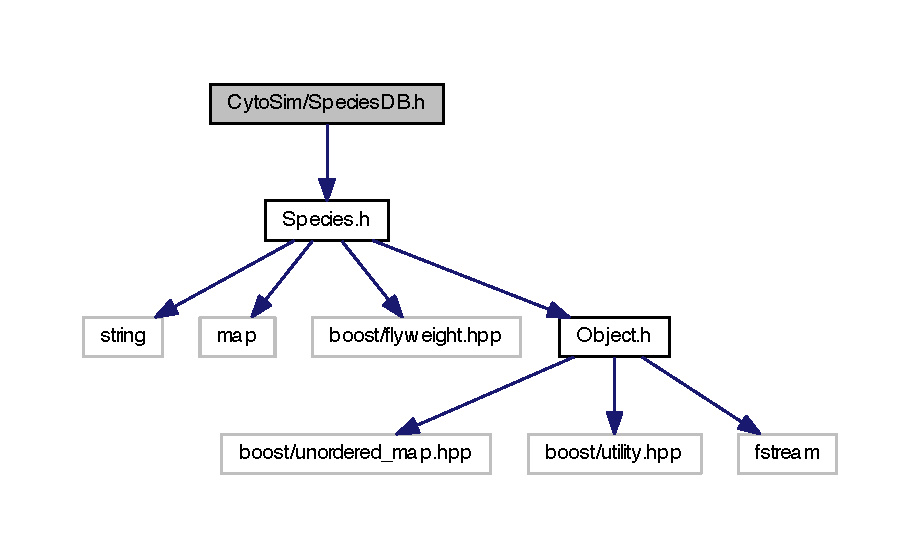
\includegraphics[width=350pt]{SpeciesDB_8h__incl}
\end{center}
\end{figure}
This graph shows which files directly or indirectly include this file\-:\nopagebreak
\begin{figure}[H]
\begin{center}
\leavevmode
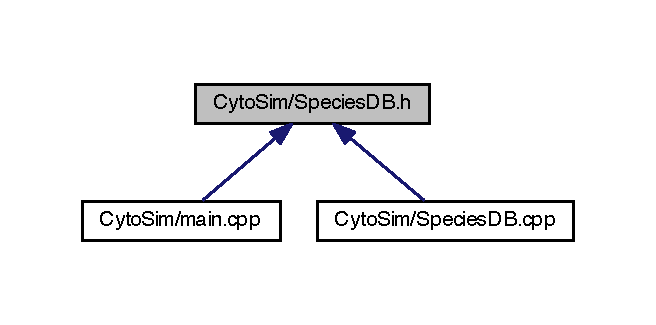
\includegraphics[width=192pt]{SpeciesDB_8h__dep__incl}
\end{center}
\end{figure}
\subsection*{Classes}
\begin{DoxyCompactItemize}
\item 
class \hyperlink{classchem_1_1SpeciesDB}{chem\-::\-Species\-D\-B}
\begin{DoxyCompactList}\small\item\em \hyperlink{classchem_1_1SpeciesDB}{Species\-D\-B} can be used to manage the lifetime of \hyperlink{classchem_1_1Species}{Species}. \end{DoxyCompactList}\end{DoxyCompactItemize}
\subsection*{Namespaces}
\begin{DoxyCompactItemize}
\item 
namespace \hyperlink{namespacechem}{chem}
\end{DoxyCompactItemize}

\printindex
\end{document}
